\chapter{Desarrollo de un generador de cargas de trabajo para sistemas publish/subscribe 
basados en contenido} \label{chp:desarrollo}

En esta sección se expone el trabajo realizado durante el desarrollo de este
generador, así como su contexto y motivación, y los resultados obtenidos.

%%%%%%%%%%%%%%%%%%%%%%%%%%%%%%%%%%%%%%%%%%%%%%%%%%%%%%%%%%%%%%%%%%%%%%%%%%%%%%%%
%%%%%%%%%%%%%%%%%%%%%%%%%%%%%%%%%%%%%%%%%%%%%%%%%%%%%%%%%%%%%%%%%%%%%%%%%%%%%%%%

\section{Motivación} \label{sct:desarrollo_motivacion}

% Necesidad de probar E-SilboPS con dataset real
La necesidad de este generador se origina en la dificultad de probar el sistema \textit{E-SilboPS}
con cargas de trabajo con datos reales (\ref{sct:art_sistpubsubcont_problemasdatasetreales}), 
habiendo sido probado solo con cargas de trabajo sintéticas (artificiales),
es decir, generadas por un programa en base a ciertos parámetros estadísticos (número de 
subscripciones totales, número de subscripciones por segundo, número de notificaciones, 
número de notificaciones por segundo, etc).

% Escasez de dataset reales (ya contado un millón de veces)
El principal problema con este tipo de pruebas es que no reflejan el comportamiento que tendrá
el sistema en un entorno real, incluso cuando las cargas generadas intentan reflejar dicho entorno.
Para solventar esto, se necesita una carga de trabajo real compatible con este sistema.

Para llevar a cabo estas pruebas con la carga de trabajo real, se necesita generar, a partir
de esta, una carga compatible con \textit{E-SilboPS}, transformando cada evento al formato aceptado
por este sistema, preservando el orden y contexto original.

%%%%%%%%%%%%%%%%%%%%%%%%%%%%%%%%%%%%%%%%%%%%%%%%%%%%%%%%%%%%%%%%%%%%%%%%%%%%%%%%
%%%%%%%%%%%%%%%%%%%%%%%%%%%%%%%%%%%%%%%%%%%%%%%%%%%%%%%%%%%%%%%%%%%%%%%%%%%%%%%%

\section{Carga de trabajo} \label{sct:desarrollo_carga}

Esta carga de trabajo se ha extraído del repositorio de \textit{datasets} del 
\textit{Middleware Systems Research Group}\footnote{\href{http://msrg.org/}{http://msrg.org/}}
de la Universidad de Toronto, y pertenece al proyecto
\textit{Mammoth}\footnote{\href{http://msrg.org/datasets/mammoth}{http://msrg.org/datasets/mammoth}},
que se ha creado por medio de obtener la información de los eventos de un juego 
\textit{MMO}\footnote{\textit{Massive Multiplayer Online Game} - Videojuego online con multitud de 
jugadores a través de Internet} que funciona mediante un sistema \textit{publish-subscribe} basado
en contenido.

Además de haberse generado a partir de un sistema similar al que se ha usado en este proyecto, es lo 
suficientemente amplia para llevar a cabo las pruebas necesarias en nuestro sistema, y presenta un
elevado número de subscripciones y de-subscripciones, cualidad necesaria para comprobar las 
fluctuaciones causadas por los incrementos y decrementos de la cantidad de trabajo recibida.

%%%%%%%%%%%%%%%%%%%%%%%%%%%%%%%%%%%%%%%%%%%%%%%%%%%%%%%%%%%%%%%%%%%%%%%%%%%%%%%%

\subsection{Análisis estático} \label{ssct:desarrollo_carga_analisis}

% Análisis del dataset
% - Análisis estático
%  + Objetivo del análisis
%  + Comparar formatos (incluir figuras con ambos formatos)

Previo uso de la carga, se ha llevado a cabo un análisis estático, con el objetivo de comprobar su
compatibilidad con el formato de los eventos de \textit{E-SilboPS} y la integridad de los propios 
datos, y, además, poder conocer de antemano datos estadísticos relevantes para el futuro desarrollo
y especificación de pruebas que la usen.

Mediante este análisis, se ha obtenido la siguiente información básica sobre la carga de trabajo:
\begin{itemize}
    \item[•] La marca de tiempo (\textit{timestamp})\footnote{En este trabajo, el término
    \textit{timestamps} y \textit{marca de tiempo} se usarán de forma intercambiable}, está
    compuesta por \texttt{13} dígitos, a diferencia de la de \textit{Linux}, de \texttt{10} dígitos.
    \item[•] Contiene mensajes de error (\texttt{[ERROR] ...}), que han de ser eliminados.
    \item[•] Tiene mensajes generados de manera simultánea, ya que el \textit{timestamp} de algunos
    mensajes es igual.
\end{itemize}

De forma adicional, se ha generado la siguiente información estadística, útil para el desarrollo 
futuro de este proyecto:
\begin{itemize}
    \item[•] Número de subscripciones: \texttt{113.904}
    \item[•] Número de de-subscripciones: \texttt{112.682}
    \item[•] Número de publicaciones: \texttt{6.207.207}
\end{itemize}

Con el objetivo de comprobar la correctitud de los eventos de la carga de trabajo, se ha verificado
que la carga no contiene subscripciones y de-subscripciones duplicadas, o de-subscripciones antes que 
la subscripción correspondiente.

%%%%%%%%%%%%%%%%%%%%%%%%%%%%%%%%%%%%%%%%%%%%%%%%%%%%%%%%%%%%%%%%%%%%%%%%%%%%%%%%

\subsection{Formato y operadores} \label{ssct:desarrollo_carga_formato}

Para concluir el análisis estático, se han comparado los formatos de cada tipo 
de eventos que, de acuerdo a la documentación de Mammoth\cite{paper:mammoth_paper} 
y E-SilboPS\cite{thesis:tesisVictor}, ambos sistemas cuentan con los siguientes
operadores para los pares clave-valor de sus eventos.

\begin{table}[htpb]
    \centering
    \begin{tabular}{|c|c|c|}
        \hline
        \textbf{E-SilboPS} & \textbf{Mammoth} & \textbf{Descripción} \\
        \hline
        \texttt{\{''exists'': ...\}}   & -  & El atributo existe \\
        \texttt{\{''='': ...\}}        & \texttt{eq} & Igual \\
        \texttt{\{''!='': ...\}}       & -  & No igual \\
        \texttt{\{''>'': ...\}}        & -  & Mayor que \\
        \texttt{\{''>='': ...\}}       & -  & Mayor o igual que \\
        \texttt{\{''<'': ...\}}        & -  & Menor que \\
        \texttt{\{''<='': ...\}}       & -  & Menor o igual que \\
        \texttt{\{''\^'': ...\}}       & -  & Comienza con el prefijo \\
        \texttt{\{''\$'': ...\}}       & -  & Termina con el sufijo \\
        \texttt{\{''contains'': ...\}} & -  & Contiene \\
        \hline
    \end{tabular}
    \caption{Tabal comparativa de operadores de \textit{E-SilboPS} y \textit{Mammoth}}
    \label{tab:comparadores}
\end{table}

Como se observa en el \autoref{tab:comparadores}, estos sistemas solo comparten el operador
de igualdad (\texttt{eq}), por lo que la carga de trabajo generada solo contendrá este operador 
para todas las pares clave-valor de cada uno de los eventos presentes en la misma.

El formato de los eventos en ambos sistemas son también diferentes entre sí para los tres tipos 
de eventos que manejan, siendo el formato de las subscripciones, como se ve en los
\autoref{lst:esilbops_sub} y \autoref{lst:mammoth_sub}, compatible, pues los 
\textit{''constraints''} son las claves y valores que se comprueban contra las publicaciones,
que en \textit{Mammoth} son los valores entre corchetes, mientras que el valor entre llaves es
el \textit{timestamp} de la subscripción, la cual solo se usará para mantener el orden de los
eventos en el fichero.\\

\begin{lstlisting}[caption={Ejemplo de subscripción de E-SilboPS.},label={lst:esilbops_sub}, style=consola,captionpos=b]
{
	"id" : "",
	"contextFunction": {},
	"constraints": {
		"symbol:str": [{"=": "GOOG"}],
		"value:double": [{">": 100.25}, {"<=": 500.0}],
		"volume:long": [{">=": 1000}],
		"timestamp:long": [{"exists": ""}]
	}
}
\end{lstlisting}

\begin{lstlisting}[caption={Ejemplo de subscripción de Mammoth.}, label={lst:mammoth_sub}, style=consola,captionpos=b]
{1307423528250} s [class,eq,broadcast] (rmi://10.0.1.2:1099/Broker2-M4894)
\end{lstlisting}

A diferencia que en \textit{Mammoth}, como se ve en \autoref{lst:esilbops_unsub} y 
\autoref{lst:mammoth_unsub}, el formato de las de-subscripciones en \textit{E-SilboPS} 
es igual al de las subscripciones. A pesar de esto, la compatibilidad se mantiene.

\begin{lstlisting}[caption={Ejemplo de de-subscripcion de E-SilboPS.},label={lst:esilbops_unsub},style=consola,captionpos=b]
{
	"id" : "",
	"contextFunction": {},
	"constraints": {
		"symbol:str": [{"=": "GOOG"}],
		"value:double": [{">": 100.25}, {"<=": 500.0}],
		"volume:long": [{">=": 1000}],
		"timestamp:long": [{"exists": ""}]
	}
}
\end{lstlisting}

\begin{lstlisting}[caption={Ejemplo de de-subscripción de Mammoth.},label={lst:mammoth_unsub},style=consola,captionpos=b]
{1307425244397} us rmi://10.0.1.4:1099/Broker4-M81393
\end{lstlisting}

En las publicaciones, el formato de ambos sistemas son muy similares y compatibles, como se puede ver
en \autoref{lst:esilbops_pub} y \autoref{lst:mammoth_pub}.

\begin{lstlisting}[caption={Ejemplo de publicación de E-SilboPS.},label={lst:esilbops_pub},style=consola,captionpos=b]
{
	 "symbol:str" : "GOOG",
	 "value:double" : 333.2,
	 "volume:long" : 345
}
\end{lstlisting}

\begin{lstlisting}[caption={Ejemplo de publicación de Mammoth.},label={lst:mammoth_pub},style=consola,captionpos=b]
{1307422272885} p [class,ProxyID_-3884500000][x,0.0][y,0.0]
\end{lstlisting}



%%%%%%%%%%%%%%%%%%%%%%%%%%%%%%%%%%%%%%%%%%%%%%%%%%%%%%%%%%%%%%%%%%%%%%%%%%%%%%%%
%%%%%%%%%%%%%%%%%%%%%%%%%%%%%%%%%%%%%%%%%%%%%%%%%%%%%%%%%%%%%%%%%%%%%%%%%%%%%%%%

\section{Diseño} \label{sct:desarrollo_diseno}

El programa deberá leer cada línea del fichero de entrada, es decir, la carga de trabajo
proveniente de \textit{Mammoth}, interpretar cada evento y generar el mismo evento en el formato 
compatible con \textit{E-SilboPS}, manteniendo los datos y el orden de los mismos. El fichero generado 
debe ser en formato \textit{JSON}\footnote{JavaScript Object Notation}, ya que es ese el
formato de los eventos de \textit{E-SilboPS}.

En este sistema, al tener las subscripciones y las de-subscripciones el mismo formato, el generador
tiene que ser capaz de guardar todas las subscripciones que haya generado, y generar las 
de-subscripciones de las mismas cuando así lo lea del fichero de entrada.

De igual forma, ha de ser capaz de detectar errores en los eventos leídos,
comprobando la correcta estructura de cada regla, sus valores, y sus operadores.

% No se me ocurre que más poner, no es tan complejo el generador

%%%%%%%%%%%%%%%%%%%%%%%%%%%%%%%%%%%%%%%%%%%%%%%%%%%%%%%%%%%%%%%%%%%%%%%%%%%%%%%%
%%%%%%%%%%%%%%%%%%%%%%%%%%%%%%%%%%%%%%%%%%%%%%%%%%%%%%%%%%%%%%%%%%%%%%%%%%%%%%%%

\section{Implementación} \label{sct:desarrollo_implementacion}

El generador se ha implementado en el lenguaje de programación
\textit{Java}\footnote{\href{https://www.java.com/en/}{https://www.java.com/en/}}, utilizando
las herramientas, \textit{Maven}\footnote{\href{https://maven.apache.org/}{https://maven.apache.org/}} 
para gestionar el proyecto y sus dependencias, y 
\textit{JUnit5}\footnote{\href{https://junit.org/junit5/}{https://junit.org/junit5/}} para realizar
pruebas y comprobar el correcto funcionamiento del programa.

A partir del diseño propuesto, se ha creado y seguido la estructura de clases que se ve en la 
\autoref{fig:parser_uml}, estableciendo una estructura de funciones transparente al usuario.

\begin{figure}[htpb]
    \centering
    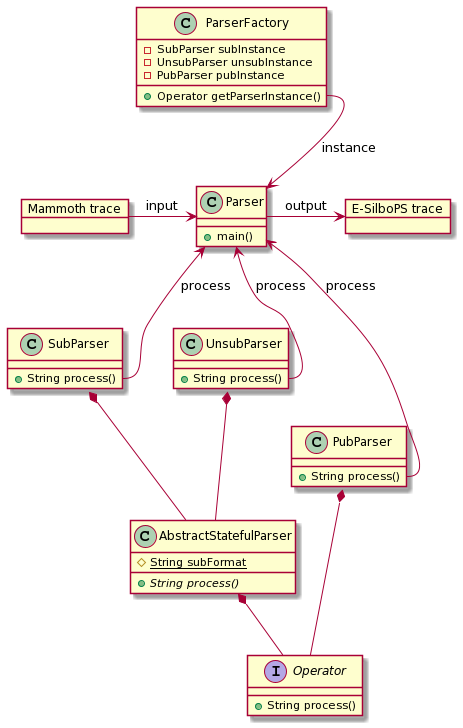
\includegraphics[width=0.75\textwidth]{images/plantuml/ParserPlantUML.png}
    \caption{Diagrama de clases del generador de cargas de trabajo reales.}
    \label{fig:parser_uml}
\end{figure}

Las clases y sus funciones mostradas en la figura \autoref{fig:parser_uml} se han simplificado para 
facilitar su lectura y comprensión general, ya que no se han incluido estructuras de datos internas
y los tipos de las mismas por ser únicamente de uso interno.

Para facilitar la lectura del fichero \textit{JSON} de salida, este se ha implementado como una lista,
o \textit{array}, de objetos \textit{JSON}, de forma que la prueba que lea dicho fichero solo tenga
que leer cada uno de estos elementos en la lista para poder usarlos, sin necesidad de realizar más
operaciones, las cuales serían necesarias si el fichero de salida no siguiese este formato.

Una vez implementado el generador, y habiendo generado el fichero \textit{JSON} que representa la carga
de trabajo real en el formato de \textit{E-SilboPS}, se puede comenzar el desarrollo de las pruebas
necesarias en este sistema usando esta carga.

%%%%%%%%%%%%%%%%%%%%%%%%%%%%%%%%%%%%%%%%%%%%%%%%%%%%%%%%%%%%%%%%%%%%%%%%%%%%%%%%
%%%%%%%%%%%%%%%%%%%%%%%%%%%%%%%%%%%%%%%%%%%%%%%%%%%%%%%%%%%%%%%%%%%%%%%%%%%%%%%%

\section{Pruebas en E-SilboPS} \label{sct:desarrollo_pruebas-esilbops}

Una vez generada la carga de trabajo deseada, se han creado las siguientes pruebas que la usan, con 
el objetivo de comprobar el comportamiento del sistema por medio de sus principales métricas de 
rendimiento, de forma que se obtenga una visión general del sistema a lo largo del tiempo.

Como no todas las publicaciones generan subscripciones, es necesario introducir dos nuevos eventos
(una subscripción al inicio (ver \autoref{lst:mammoth_subflag}), y una publicación al final 
(ver \autoref{lst:mammoth_pubflag})), a la carga, que solo se enviará una única vez, marcando el
final de la prueba correspondiente.

\begin{minipage}[t]{.5\textwidth}
\begin{lstlisting}[caption={Subscripción en E-SilboPS para identificar el final de la carga.}, label={lst:mammoth_subflag}, style=consola,captionpos=b]
{
	"id" : "MAMMOTH_FLAG"
	"contextFunction" : {},
	"constraints" : {
		"class:str" : [{"=" : "END"}]
	}
}
\end{lstlisting}
\end{minipage}
\hfill
\begin{minipage}[t]{.45\textwidth}
\begin{lstlisting}[caption={Publicación en E-SilboPS que marca el final de la carga.}, label={lst:mammoth_pubflag}, style=consola,captionpos=b]
{
    "id:long" : 0
    "class:str" : "END"
}
\end{lstlisting}
\end{minipage}

Una vez diseñados e implementados estos conceptos, se han implementado las 
siguientes pruebas, usando una topología 1-1-1 (1 EP, 1 M, 1 EP) en E-SilboPS,
siendo el emisor y el receptor diferentes hilos (\textit{threads}) de un mismo
computador.

%%%%%%%%%%%%%%%%%%%%%%%%%%%%%%%%%%%%%%%%%%%%%%%%%%%%%%%%%%%%%%%%%%%%%%%%%%%%%%%%

\subsection{Velocidad fija de envío} \label{ssct:desarrollo_pruebas-esilbops_test-fixed}

Para esta primera prueba, se ha procedido al envío de toda la carga de trabajo,
subscripciones, de-subscripciones y publicaciones, a diferentes velocidades
de envío (ver lista a continuación) mediante repetir esta prueba con cada una
de ellas.

\begin{itemize}
    \item 50.000 mensajes por segundo.
    \item 100.000 mensajes por segundo.
    \item 200.000 mensajes por segundo.
    \item 500.000 mensajes por segundo.
    \item 1.000.000 mensajes por segundo.
    \item 6.433.794 mensajes por segundo (máxima velocidad posible).
\end{itemize}

Parámetros adicionales de estas pruebas:
\begin{itemize}
    \item Número de publicaciones: 6.207.207
    \item Número de subscripciones: 113.904
    \item Número de de-subscripciones: 112.682
    \item Número de notificaciones: 4.515.781 (72\% de las publicaciones machean)
    \item Cada publicación machea como máximo, con una única subscripción.\footnote{Esto
    se tendrá en cuenta para el desarrollo de futuras pruebas.}
\end{itemize}

Para poder obtener los datos más precisos, se ha decidido medir el tiempo de respuesta una vez cada 
50.000 notificaciones recibidas\footnote{Esta característica se ha mantenido en todas las pruebas 
realizadas}, ya que medir más frecuentemente provoca una distorsión en las mediciones y por
ende, en su interpretación.

%%%%%%%%%%%%%%%%%%%%%%%%%%%%%%%%%%%%%%%%%%%%%%%%%%%%%%%%%%%%%%%%%%%%%%%%%%%%%%%%

\subsection{Secuencia logarítmica de subscripciones} \label{ssct:desarrollo_pruebas-esilbops_test-log}

En esta prueba, se separan las subscripciones y las publicaciones, enviando las subscripciones
siguiendo una secuencia logarítmica (comenzando en 100 subscripciones), hasta haber enviado todas
las subscripciones (113.904). Este proceso se muestra en la \autoref{fig:testlog-uml}). 
Tras enviar las nuevas subscripciones, se envían todas las publicaciones de la carga, midiendo el
throughput total del sistema.

Parámetros de la prueba:
\begin{itemize}
    \item Número de publicaciones: 6.207.207
    \item Subscripciones en secuencia logarítmica, de 100 a 113.904 (todas las subscripciones)
    \item La prueba se repetirá 10 veces por cada punto en la gráfica, siendo el valor final
    de este la media del throughput total de cada repetición.
    \item Velocidad de envío (input rate): 100.000 mensajes por segundo.
\end{itemize}

\begin{figure}[htpb]
    \centering
    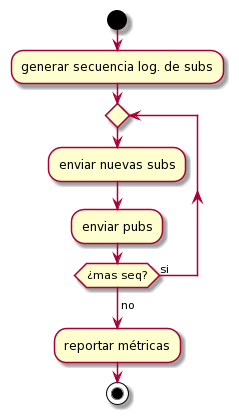
\includegraphics[width=0.35\textwidth]{images/plantuml/testlog-plantuml.png}
    \caption{Diagrama de ejecución de prueba con subscripciones en secuencia logarítmica.}
    \label{fig:testlog-uml}
\end{figure}

%%%%%%%%%%%%%%%%%%%%%%%%%%%%%%%%%%%%%%%%%%%%%%%%%%%%%%%%%%%%%%%%%%%%%%%%%%%%%%%%

\subsection{Carga de subscripciones creciente} \label{subsct:desarrollo_pruebas-esilbops_test-inc}

Para llevar a cabo esta prueba, primero se ha generado una traza de números 
(ver \autoref{fig:subs_workload-growing}) con un incremento constante hasta 
llegar a un número deseado, y manteniendo dicho número hasta el final de la misma.

Esta traza de números (\autoref{fig:subs_workload-growing}) representa el 
número de subscripciones presentes en cada momento (ver 
\autoref{sct:art_workloads}), con cierto ruido/fluctuaciones, simulando un
entorno real con nuevas subscripciones y de-subscripciones cada segundo.

Parámetros de la prueba:
\begin{itemize}
    \item Subscripciones base: 10.000
    \item Subscripciones finales: 20.000
    \item Ruido: $\pm$ 2000 subscripciones
    \item Tiempo de la prueba: 600 segundos
    \item Velocidad de envío (input rate): 50.000 mensajes por segundo
\end{itemize}

\begin{figure}[htpb]
    \centering
    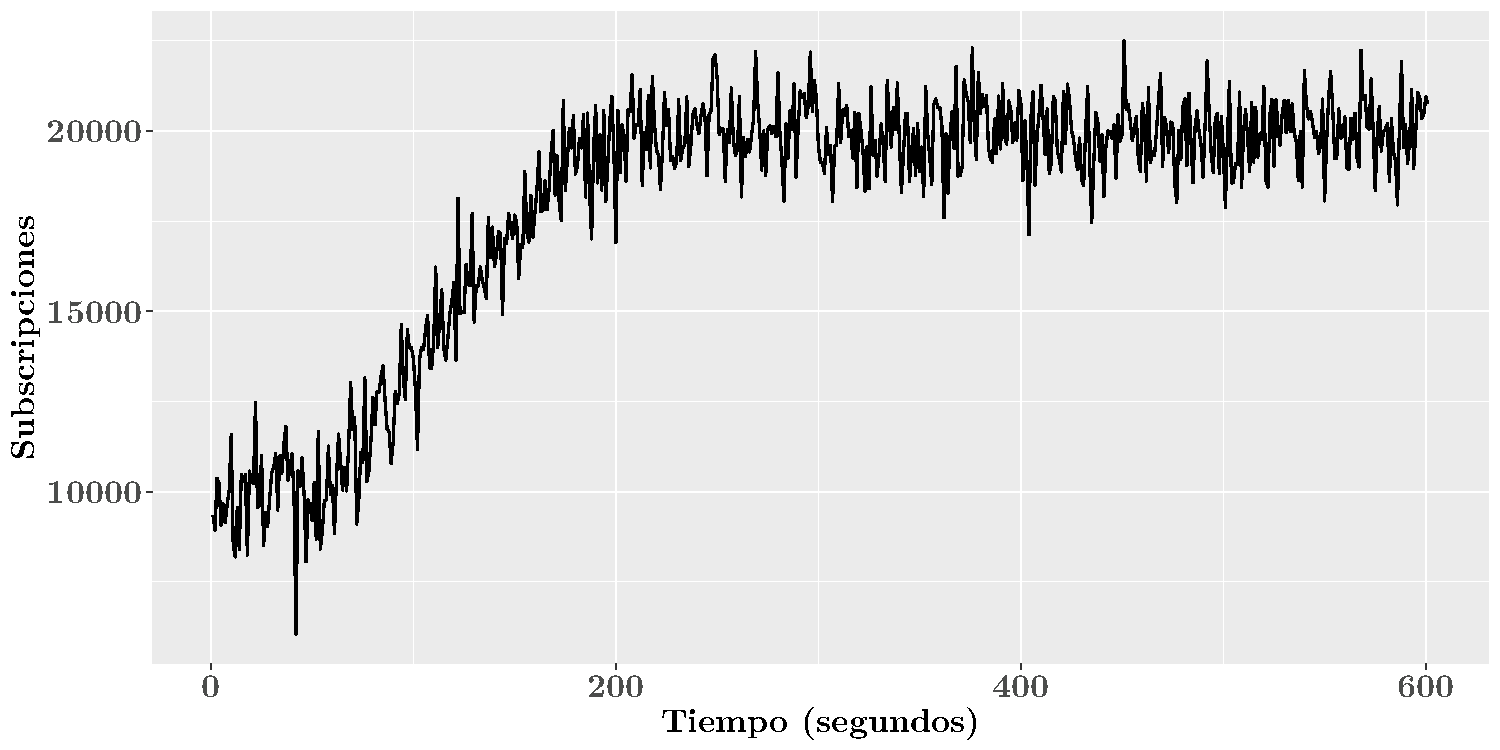
\includegraphics[width=\textwidth]{images/workload-types/subs_workload-growing.pdf}
    \caption{Ejemplo de carga de trabajo creciente (con ruido añadido).}
    \label{fig:subs_workload-growing}
\end{figure}

% Introducir el resto de trazas de este tipo (nonoise, unique-pub, unique-pubsub)

Esta traza es leída por la prueba, y, en base al número presente de subscripciones en el sistema,
genera nuevas subscripciones o de-subscripciones, de forma que, cada segundo, el sistema contenga
el número de subscripciones especificadas en esta, siguiendo el flujo de ejecución que se muestra 
en la \autoref{fig:testinc-uml}).

El envío de publicaciones se realiza a un ratio fijo por segundo (input rate), y de forma paralela al envío de 
subscripciones/de-subscripciones, interpretando las publicaciones como una lista circular hasta
que se haya recorrido toda la traza de subscripciones. Una vez esto sucede, se envían las restantes 
publicaciones y finaliza la prueba.

\begin{figure}[htpb]
    \centering
    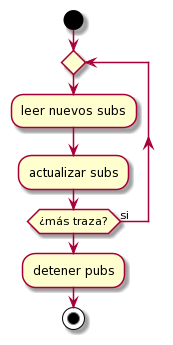
\includegraphics[width=0.35\textwidth]{images/plantuml/testinc-plantuml.png}
    \caption{Diagrama de ejecución de la prueba con carga de trabajo incremental.}
    \label{fig:testinc-uml}
\end{figure}

\subsection{Carga de subscripciones estática} \label{subsct:desarrollo_pruebas-esilbops_test-static}

Estas pruebas se han basado en la confección de una carga de trabajo basada en
la real (ver \autoref{sct:art_workloads}, \textit{Carga estática}), 
en la cual la cantidad de subscriptores no cambia durante toda la 
ejecución de dicha prueba, es decir, se envía un número determinado de subscripciones
al inicio de la prueba, y se mantienen esas subscripciones hasta acabar esta.

Junto con estas carga, se debe de especificar la velocidad a la que el sistema 
envía las publicaciones (input rate), para simular un entorno en el que el 
sistema recibe muchos eventos por segundo, que han de ser procesados y enviados,
con el objetivo de ver el punto en el que el sistema satura parcialmente.

En estas pruebas, el ratio al que se envían las publicaciones será mayor que en 
las siguientes pruebas, ya que el sistema no está procesando nuevas subscripciones
o desubscripciones, solo publicaciones entrantes.

Parámetros de las pruebas:
\begin{itemize}
    \item Dos pruebas, una con 50.000 subscripciones, otra con 100.000 subscripciones
    \item Tiempo de la prueba: 600 segundos
    \item Velocidad de envío (input rate): 200.000 mensajes por segundo
\end{itemize}

\subsection{Carga de subscripciones con crecimiento puntual} \label{subsct:desarrollo_pruebas-esilbops_test-spike}

Siguiendo con estas pruebas, se han desarrollado unas cargas de trabajo que presentan
un incremento de las subscripciones puntual, es decir, las subscripciones comienzan
constantes, y tras un periodo de tiempo, incrementan hasta cierto valor. Una vez se
llega a ese valor, todas esas nueva subscripciones se eliminan mediante el envío de
las desubscripciones correspondientes.

Subscripciones de las pruebas:
\begin{itemize}
    \item Crecimiento de 20.000 a 100.000 subscripciones (\autoref{fig:subsworkload_20k-100k})
    \item Crecimiento de 25.000 a 113.904 subscripciones (\autoref{fig:subsworkload_25k-113k})
    \item Crecimiento rápido de 25.000 a 113.904 subscripciones (\autoref{fig:subsworkload_fast_spike_25k-113k-100k})
\end{itemize}

Parámetros de las pruebas:
\begin{itemize}
    \item Publicaciones: buffer circular de 6.207.207 publicaciones
    \item Velocidad de envío (input rate): 125.000 mensajes por segundo
\end{itemize}

\begin{figure}[htpb]
    \centering
    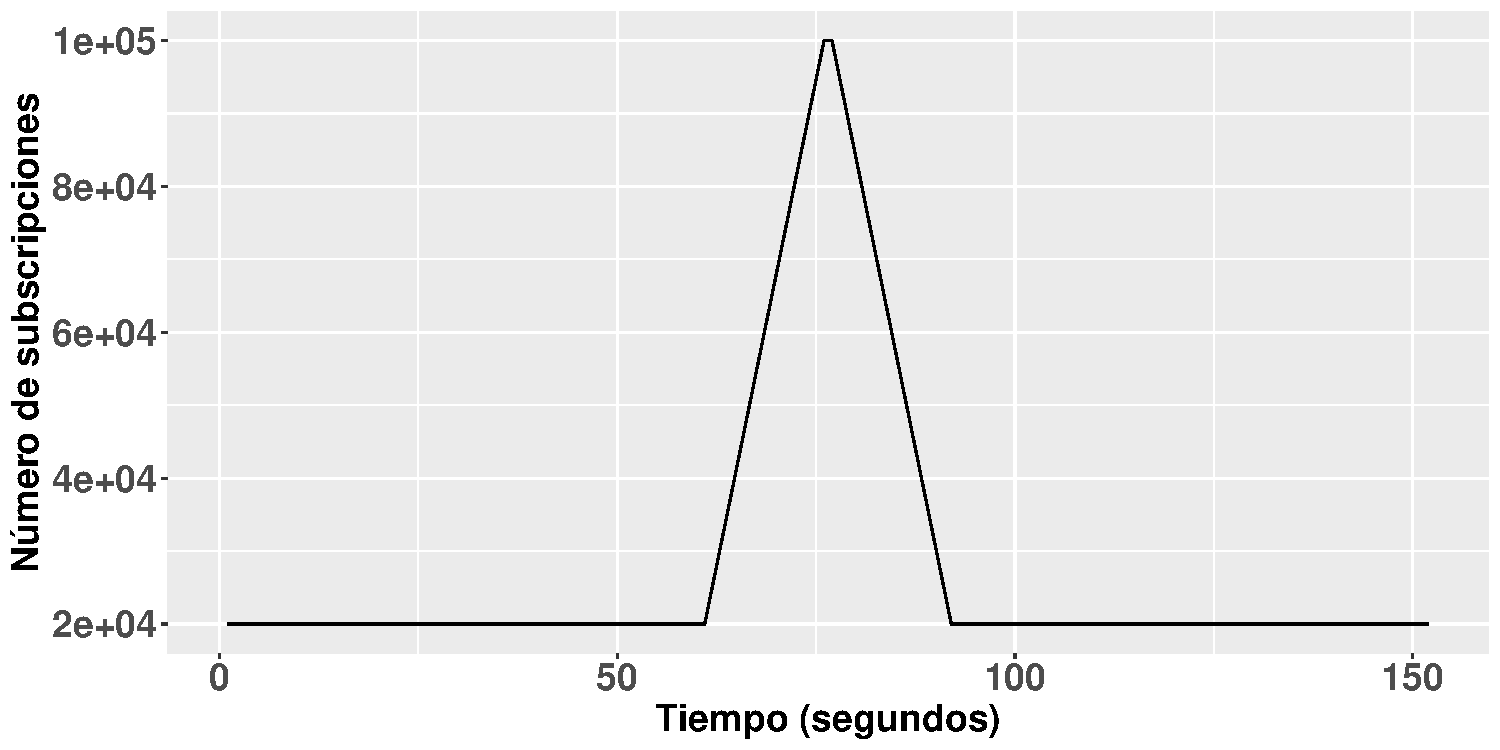
\includegraphics[width=\textwidth]{images/subs_workload_spike_20k-100k.pdf}
    \caption{Carga base de 20.000 subscripciones con incremento hasta 100.000 subscripciones.}
    \label{fig:subsworkload_20k-100k}
\end{figure}

\begin{figure}[htpb]
    \centering
    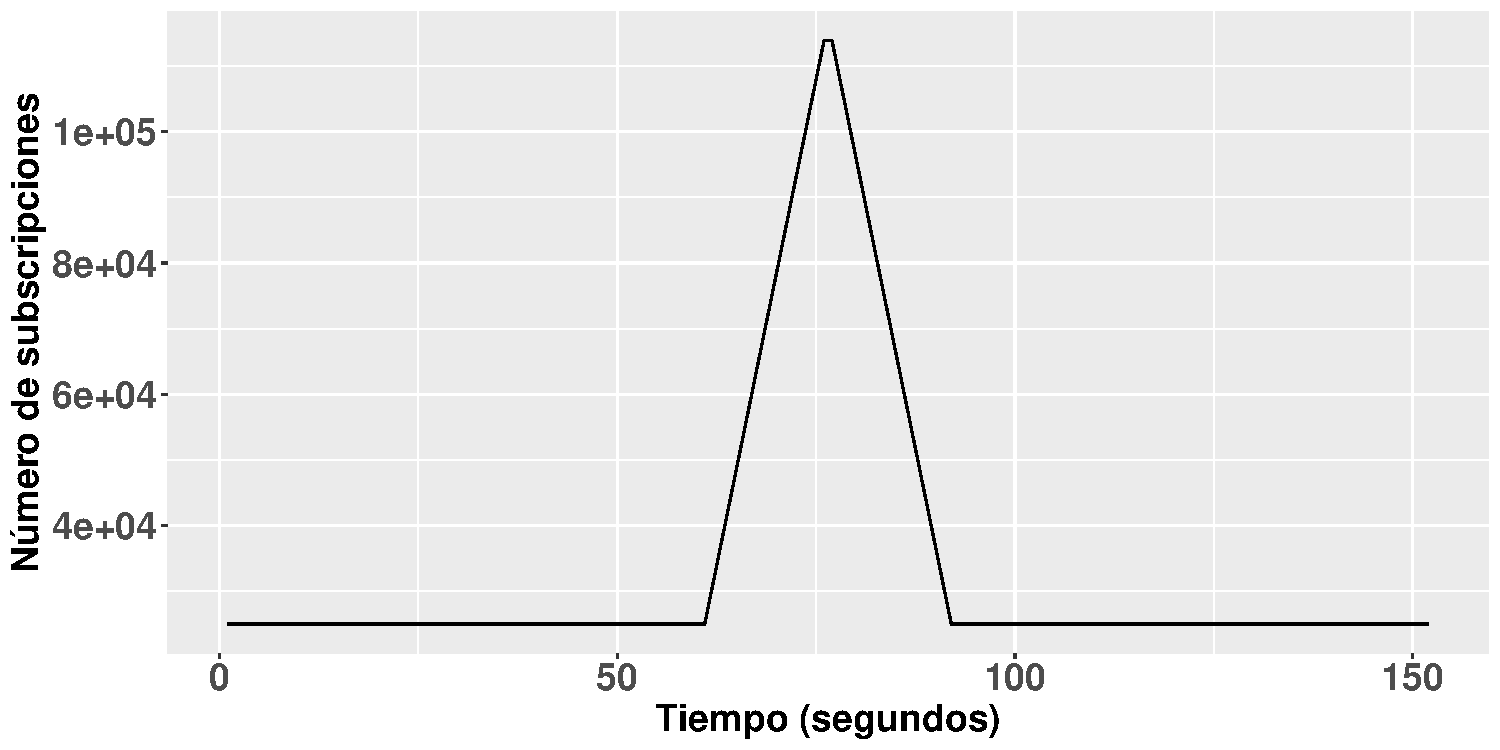
\includegraphics[width=\textwidth]{images/subs_workload_spike_25k-113k.pdf}
    \caption{Carga base de 25.000 subscripciones con incremento hasta 113.904 subscripciones.}
    \label{fig:subsworkload_25k-113k}
\end{figure}

\begin{figure}[htpb]
    \centering
    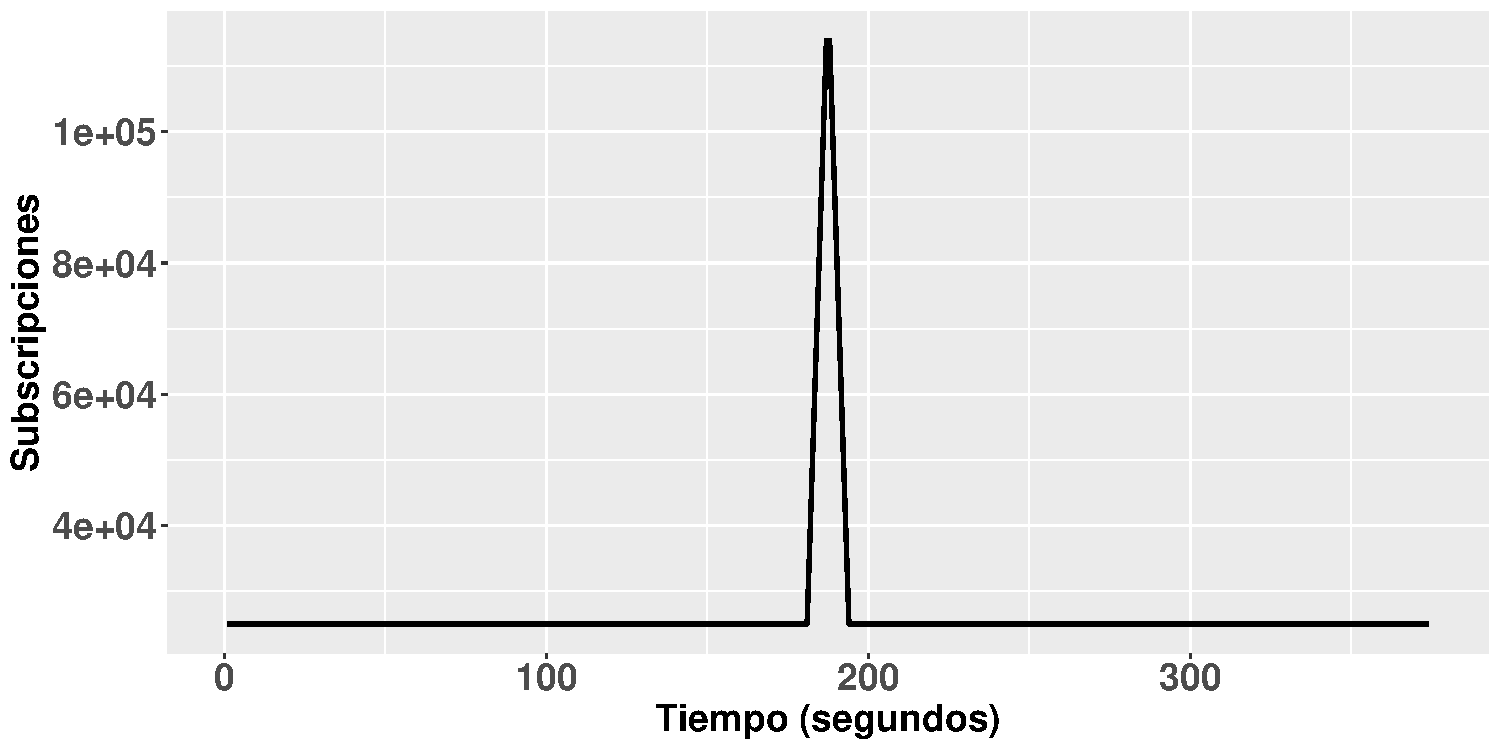
\includegraphics[width=\textwidth]{images/subs_workload_test_spike_fast_25k-113k.pdf}
    \caption{Carga base de 25.000 subscripciones con incremento muy rápido hasta 113.904 subscripciones.}
    \label{fig:subsworkload_fast_spike_25k-113k-100k}
\end{figure}



%%%%%%%%%%%%%%%%%%%%%%%%%%%%%%%%%%%%%%%%%%%%%%%%%%%%%%%%%%%%%%%%%%%%%%%%%%%%%%%%
%%%%%%%%%%%%%%%%%%%%%%%%%%%%%%%%%%%%%%%%%%%%%%%%%%%%%%%%%%%%%%%%%%%%%%%%%%%%%%%%

\section{Métricas de rendimiento} \label{sct:desarrollo_metricas}

Para poder cuantificar y analizar el rendimiento del sistema, como se ha mencionado previamente, 
es necesario obtener las principales métricas de rendimiento, con el objetivo de identificar posibles 
problemas o ineficiencias en el sistema.

Estas métricas son:
\begin{itemize}

    \item \textbf{Tiempo de respuesta} (\textit{response time}): lapso de tiempo
    desde que se envía la publicación hasta que es recibida por un usuario 
    interesado en ella.

    \item \textbf{Notificaciones enviadas a usuarios por segundo}
    (\textit{throughput}): número de notificaciones, por segundo, que han salido
    del sistema hacia usuarios interesados en ellas

\end{itemize}

Para obtener estos datos, las pruebas implementadas en la 
\autoref{sct:desarrollo_pruebas-esilbops} han recogido los tiempos de envío y 
recepción de cada mensaje, mediante los cuales se han calculado los tiempos de 
respuesta de cada publicación (que ha llegado a algún subscriptor), y el número
de mensajes totales del sistema, plasmando esta información en ficheros con el 
formato \textit{CSV}\footnote{Comma-Separated Values} para poder dibujar 
gráficas y obtener conclusiones de las pruebas y del sistema.

%%%%%%%%%%%%%%%%%%%%%%%%%%%%%%%%%%%%%%%%%%%%%%%%%%%%%%%%%%%%%%%%%%%%%%%%%%%%%%%%
%%%%%%%%%%%%%%%%%%%%%%%%%%%%%%%%%%%%%%%%%%%%%%%%%%%%%%%%%%%%%%%%%%%%%%%%%%%%%%%%

\section{Análisis de los resultados} \label{sct:desarrollo_resultados}

Con los datos obtenidos por medio de las pruebas implementadas y ejecutadas en la 
\autoref{sct:desarrollo_pruebas-esilbops}, se han obtenido los siguientes datos y 
gráficas\footnote{Ejes Y en escala logarítmica para mejor representación de los datos.}.

%%%%%%%%%%%%%%%%%%%%%%%%%%%%%%%%%%%%%%%%%%%%%%%%%%%%%%%%%%%%%%%%%%%%%%%%%%%%%%%%

\subsection*{Velocidad fija de envío}

Esta prueba, como se ha mencionado en la \autoref{ssct:desarrollo_pruebas-esilbops_test-fixed},
se ha llevado a cabo múltiples veces a diferentes velocidades de envío (input rate), para poder
ver el comportamiento del sistema, tanto en throughput como en tiempo de respuesta de notificación.

%%%%%%%%%%%%%%%%%%%%%%%%%%%%%%%%%%%%%%%%%%%%%%%%%%%%%%%%%%%%%%%%%%%%%%%%%%%%%%%%

\subsubsection*{- 50.000 mensajes por segundo}

Los resultados de esta prueba, tanto del throughput (ver 
\autoref{fig:fullworkload-inc-msgrate-th-50k}) como del 
tiempo de respuesta (ver \autoref{fig:fullworkload-inc-msgrate-rt-50k}) 
muestran un sistema que funciona sin saturar, pues el tiempo de respuesta es 
muy cercano a 0. 
El throughput muestra ciertos picos precedidos de valles, los cuales se deben 
al propio contenido de la carga de trabajo ya que hay zonas que provocan más 
subscripciones que otras, y no llega a las 50.000 notificaciones por segundo
(salvo en los ya mencionados picos), debido a que no todas las publicaciones 
producen alguna notificación.

Conclusiones de la prueba
\begin{itemize}
    \item Tiempo de respuesta mínimo y estable
    \item Throughput por debajo del input rate (esperable), picos debidos a la propia carga.
\end{itemize}

\begin{figure}[htpb]
    \centering
    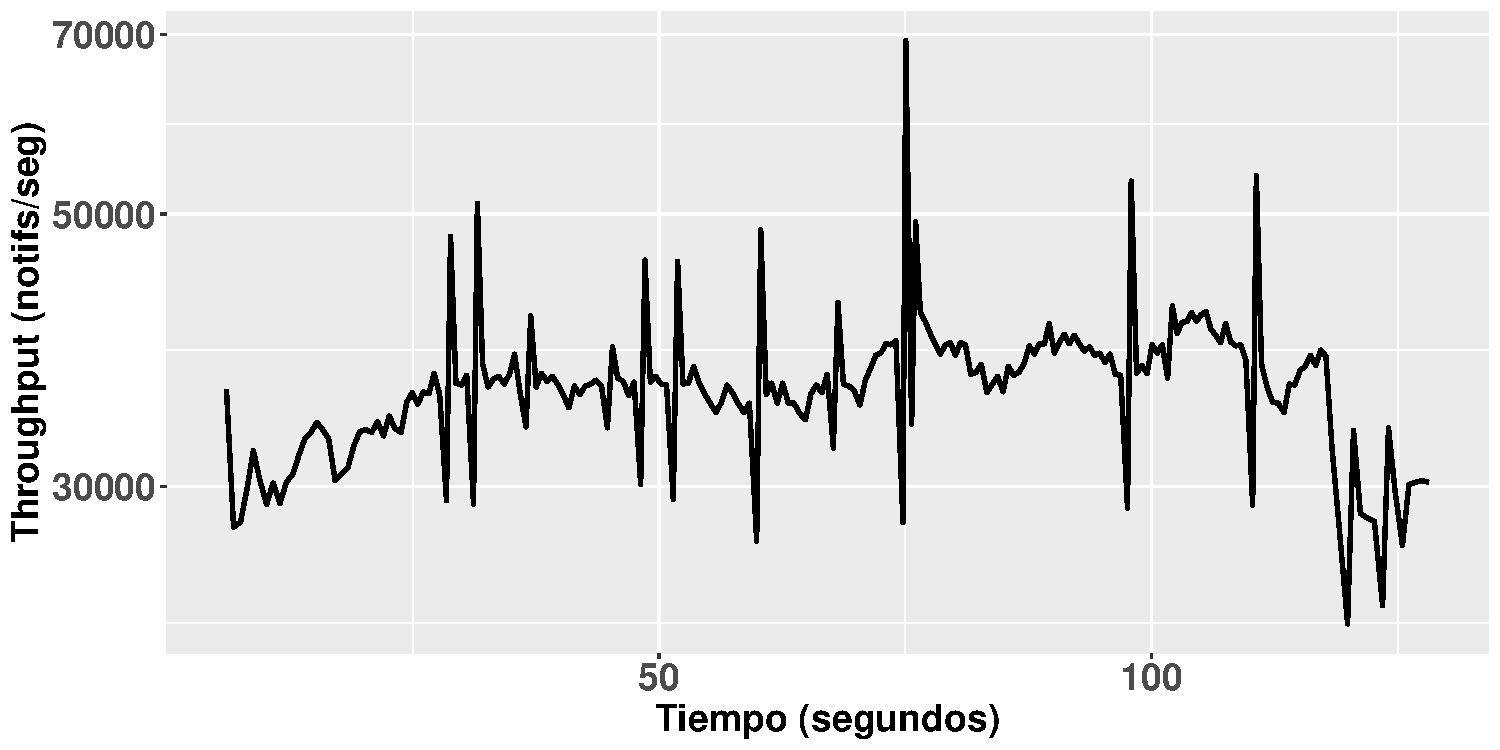
\includegraphics[width=\textwidth]{images/full-worklad-inc-msgrate/th_full-workload-inc-msgrate_50k.pdf}
    \caption{Throughput de prueba con carga completa e input rate de 50.000 mensajes/s.}
    \label{fig:fullworkload-inc-msgrate-th-50k}
\end{figure}

\begin{figure}[htpb]
    \centering
    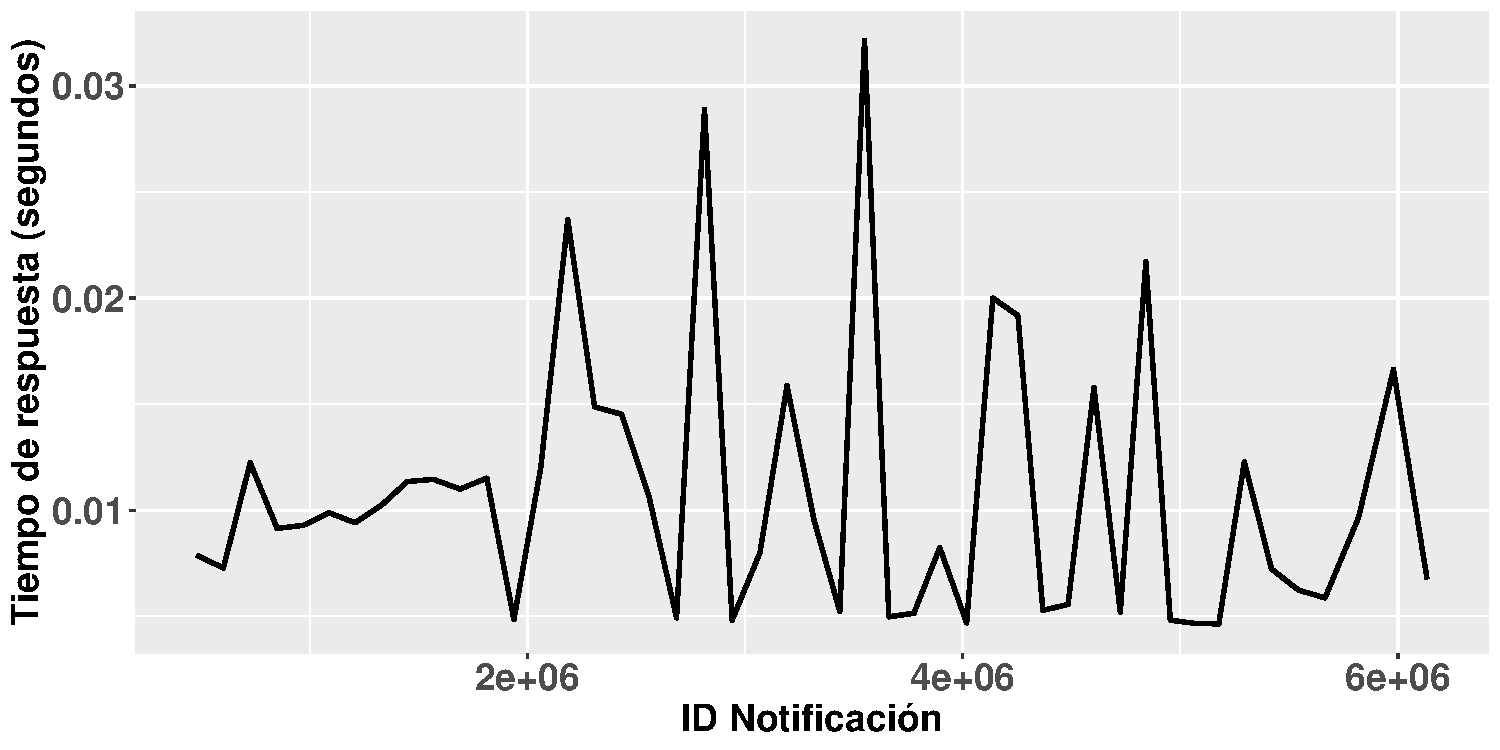
\includegraphics[width=\textwidth]{images/full-worklad-inc-msgrate/rt_full-workload-inc-msgrate_50k.pdf}
    \caption{Tiempo de respuesta de prueba con carga completa e input rate de 50.000 mensajes/s.}
    \label{fig:fullworkload-inc-msgrate-rt-50k}
\end{figure}

%%%%%%%%%%%%%%%%%%%%%%%%%%%%%%%%%%%%%%%%%%%%%%%%%%%%%%%%%%%%%%%%%%%%%%%%%%%%%%%%

\subsubsection*{- 100.000 mensajes por segundo}

Los resultados de esta prueba, tanto en el throughput (ver 
\autoref{fig:fullworkload-inc-msgrate-th-100k}) como en el tiempo de respuesta
(ver \autoref{fig:fullworkload-inc-msgrate-rt-100k}), muestran que el sistema ha
saturado de forma parcial, ya que el throughput cae muy por debajo del valor
esperado, y el tiempo de respuesta crece de forma constante, lo que indica que
el sistema no está procesando las publicaciones a tiempo, y se están encolando.

Además de esto, se puede ver claramente la relación entre ambas mediciones,
ya que la caída del throughput (\autoref{fig:fullworkload-inc-msgrate-th-100k},
a los 50 segundos), concuerda con el incremento en el tiempo de respuesta
(\autoref{fig:fullworkload-inc-msgrate-rt-100k} a partir de la notificación
con ID 3.000.000).

Conclusiones de la prueba:
\begin{itemize}
    \item El tiempo de respuesta crece de forma constante, ya que se encolan las
    notificaciones.
    \item El sistema satura de forma parcial, debido al throughput inestable, llegando
    a caer hasta los 3.000 mensajes por segundo.
\end{itemize}

\begin{figure}[htpb]
    \centering
    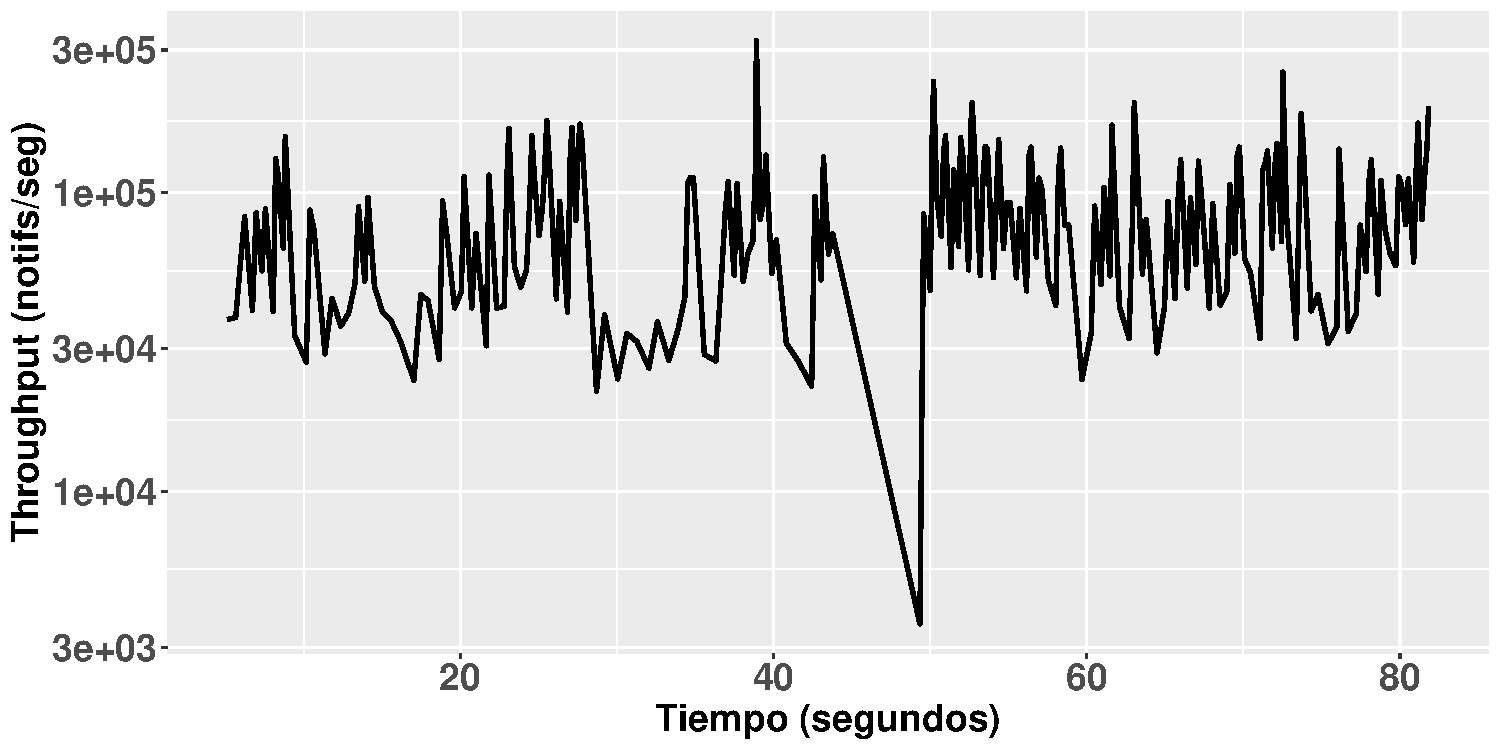
\includegraphics[width=\textwidth]{images/full-worklad-inc-msgrate/th_full-workload-inc-msgrate_100k.pdf}
    \caption{Throughput de prueba con carga completa e input rate de 100.000 mensajes/s.}
    \label{fig:fullworkload-inc-msgrate-th-100k}
\end{figure}

\begin{figure}[htpb]
    \centering
    \includegraphics[width=\textwidth]{images/full-worklad-inc-msgrate/rt_full-workload-inc-msgrate_100k.pdf}
    \caption{Tiempo de respuesta de prueba con carga completa e input rate de 100.000 mensajes/s.}
    \label{fig:fullworkload-inc-msgrate-rt-100k}
\end{figure}

%%%%%%%%%%%%%%%%%%%%%%%%%%%%%%%%%%%%%%%%%%%%%%%%%%%%%%%%%%%%%%%%%%%%%%%%%%%%%%%%

\subsubsection*{- 200.000 mensajes por segundo}

% explicaciones
En esta prueba, los resultados del throughput (ver 
\autoref{fig:fullworkload-inc-msgrate-th-200k}) y del tiempo de respuesta (ver
\autoref{fig:fullworkload-inc-msgrate-rt-200k}, demuestran que el sistema ha 
saturado, pero su throughput no ha caído tanto como anteriormente, a diferencia
del tiempo de respuesta, que sí ha crecido en gran medida, lo cual indica que las
notificaciones se están encolando en gran medida, ya que el sistema no puede 
procesarlas a tiempo, llegando estas a llegar al cliente tras más de 40 segundos.

Conclusiones de la prueba:
\begin{itemize}
    \item El tiempo de respuesta se incrementa de forma exponencial.
    \item El throughput presenta muchos picos al encolar muchas notificaciones que
    se procesan de forma muy rápida, llegando algunos picos a superar el input rate.
\end{itemize}

\begin{figure}[htpb]
    \centering
    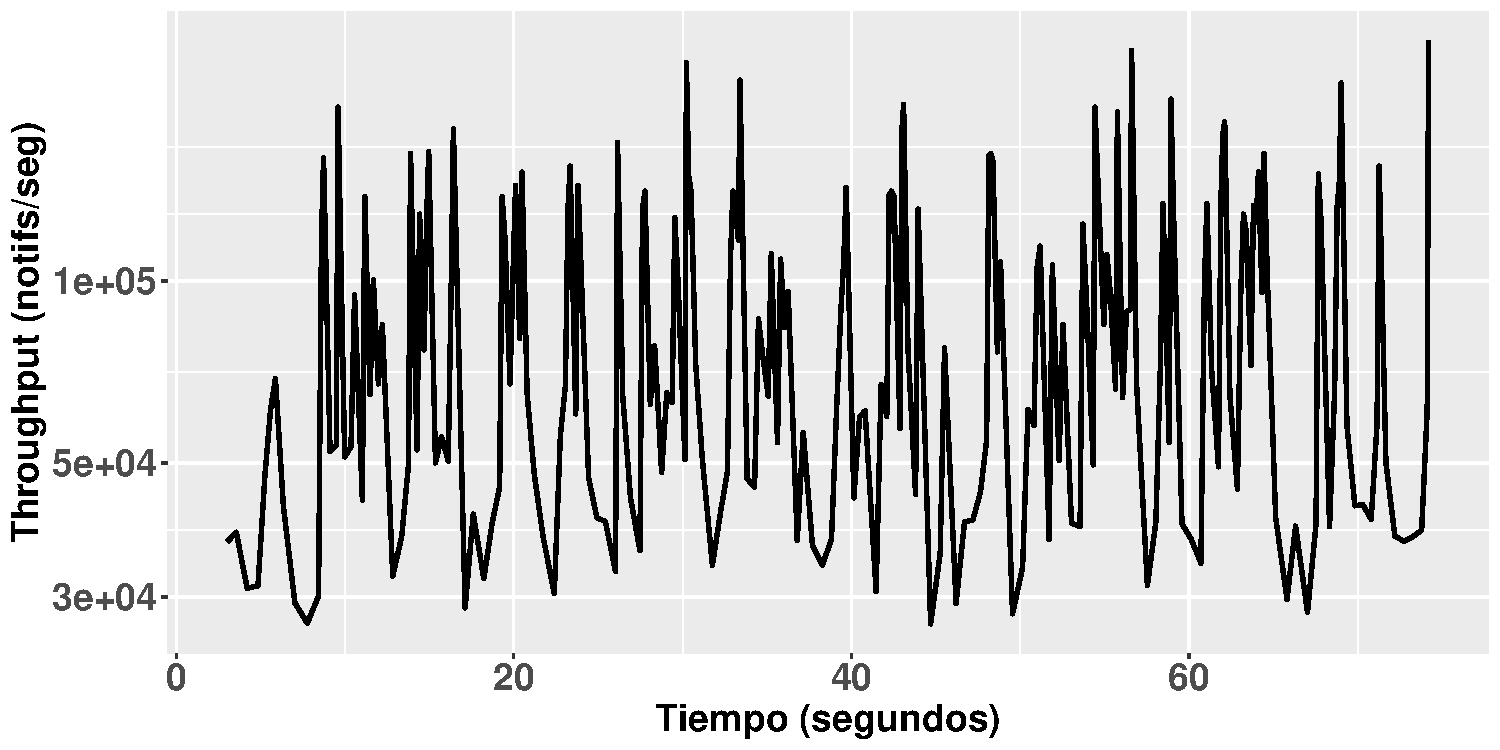
\includegraphics[width=\textwidth]{images/full-worklad-inc-msgrate/th_full-workload-inc-msgrate_200k.pdf}
    \caption{Throughput de prueba con carga completa e input rate de 200.000 mensajes/s.}
    \label{fig:fullworkload-inc-msgrate-th-200k}
\end{figure}

\begin{figure}[htpb]
    \centering
    \includegraphics[width=\textwidth]{images/full-worklad-inc-msgrate/rt_full-workload-inc-msgrate_200k.pdf}
    \caption{Tiempo de respuesta de prueba con carga completa e input rate de 200.000 mensajes/s.}
    \label{fig:fullworkload-inc-msgrate-rt-200k}
\end{figure}

%%%%%%%%%%%%%%%%%%%%%%%%%%%%%%%%%%%%%%%%%%%%%%%%%%%%%%%%%%%%%%%%%%%%%%%%%%%%%%%%

\subsubsection*{- 500.000 mensajes por segundo}

% explicaciones
Al igual que en las pruebas anteriores, se puede ver la saturación del sistema,
tanto en el throughput (ver \autoref{fig:fullworkload-inc-msgrate-th-500k})
como en el tiempo de respuesta (ver \autoref{fig:fullworkload-inc-msgrate-rt-500k}),
presentando en el primero importantes caídas (hasta casi 3.000 de throughput),
y un tiempo de respuesta que llega a casi 70 segundos. 

En esta prueba también se puede apreciar la relación del throughput y del
tiempo de respuesta, pues este último presenta dos repentinos incrementos, los cuales
coinciden con severas caídas del throughput.

Conclusiones de la prueba:
\begin{itemize}
    \item El tiempo de respuesta es mucho mayor que en anteriores pruebas, señal
    del grado de saturación del sistema.
    \item El throughput muestra severas caídas, y oscila en torno a los 100.000
    mensajes por segundo, muy por debajo de los 500.000 de input rate.
\end{itemize}

\begin{figure}[htpb]
    \centering
    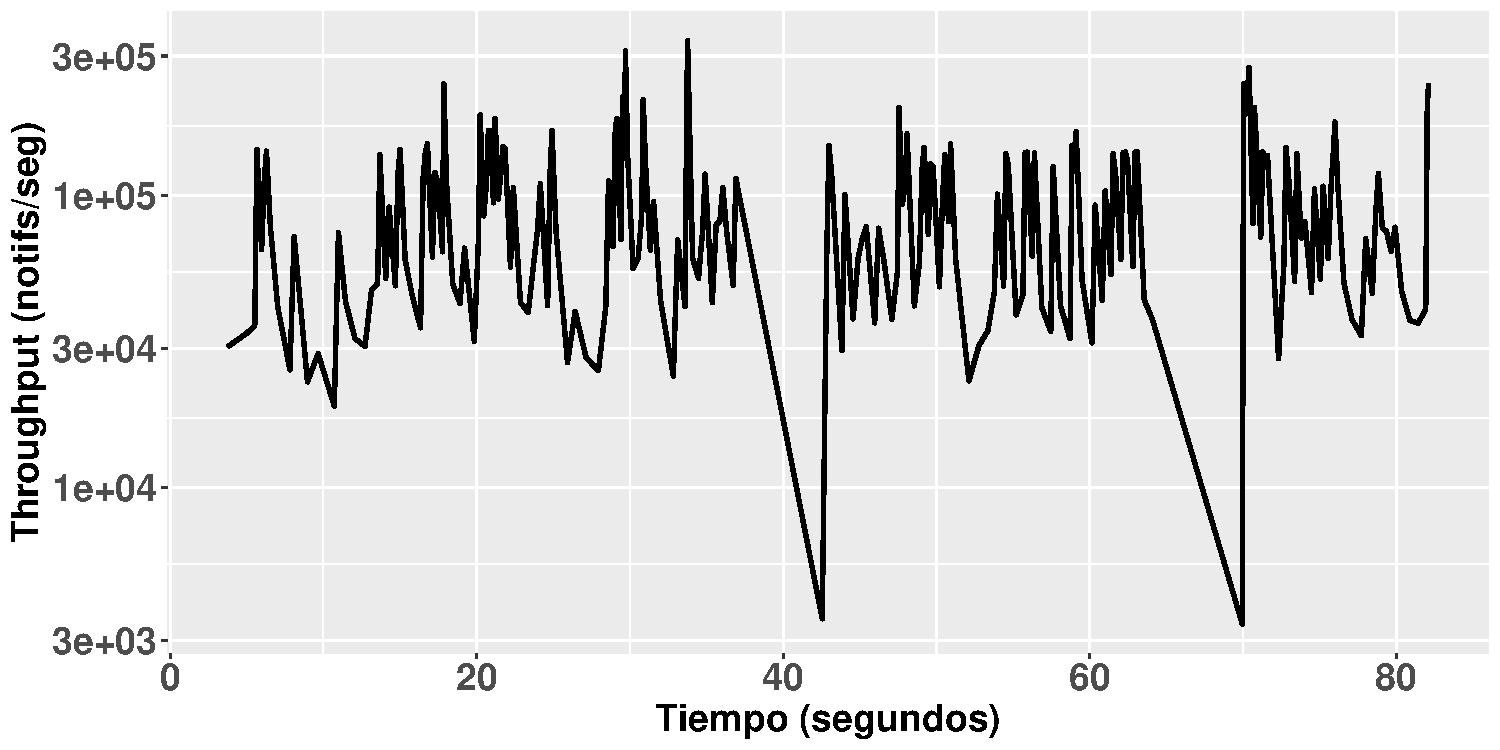
\includegraphics[width=\textwidth]{images/full-worklad-inc-msgrate/th_full-workload-inc-msgrate_500k.pdf}
    \caption{Throughput de prueba con carga completa e input rate de 500.000 mensajes/s.}
    \label{fig:fullworkload-inc-msgrate-th-500k}
\end{figure}

\begin{figure}[htpb]
    \centering
    \includegraphics[width=\textwidth]{images/full-worklad-inc-msgrate/rt_full-workload-inc-msgrate_500k.pdf}
    \caption{Tiempo de respuesta de prueba con carga completa e input rate de 500.000 mensajes/s.}
    \label{fig:fullworkload-inc-msgrate-rt-500k}
\end{figure}

%%%%%%%%%%%%%%%%%%%%%%%%%%%%%%%%%%%%%%%%%%%%%%%%%%%%%%%%%%%%%%%%%%%%%%%%%%%%%%%%

\subsubsection*{- 1.000.000 mensajes por segundo}

Los resultados de esta prueba son muy similares a los de la prueba anterior,
con un throughput (ver \autoref{fig:fullworkload-inc-msgrate-th-1M}) con muchos
picos alrededor de 75.000 mensajes por segundo, y que presenta 3 caídas severas,
las cuales coinciden con 3 incrementos presentes en el tiempo de respuesta (ver
\autoref{fig:fullworkload-inc-msgrate-rt-1M}), el cual presenta mayores valores
que en las pruebas anteriores.

Conclusiones de la prueba:
\begin{itemize}
    \item El throughput presenta serias caídas (hasta los 3.000 mensajes por segundo),
    y no llega a los 300.000 mensajes por segundo.
    \item El tiempo de respuesta denota la saturación del sistema, llegando hasta
    los 80 segundos de espera en la llegada de las notificaciones.
\end{itemize}

\begin{figure}[htpb]
    \centering
    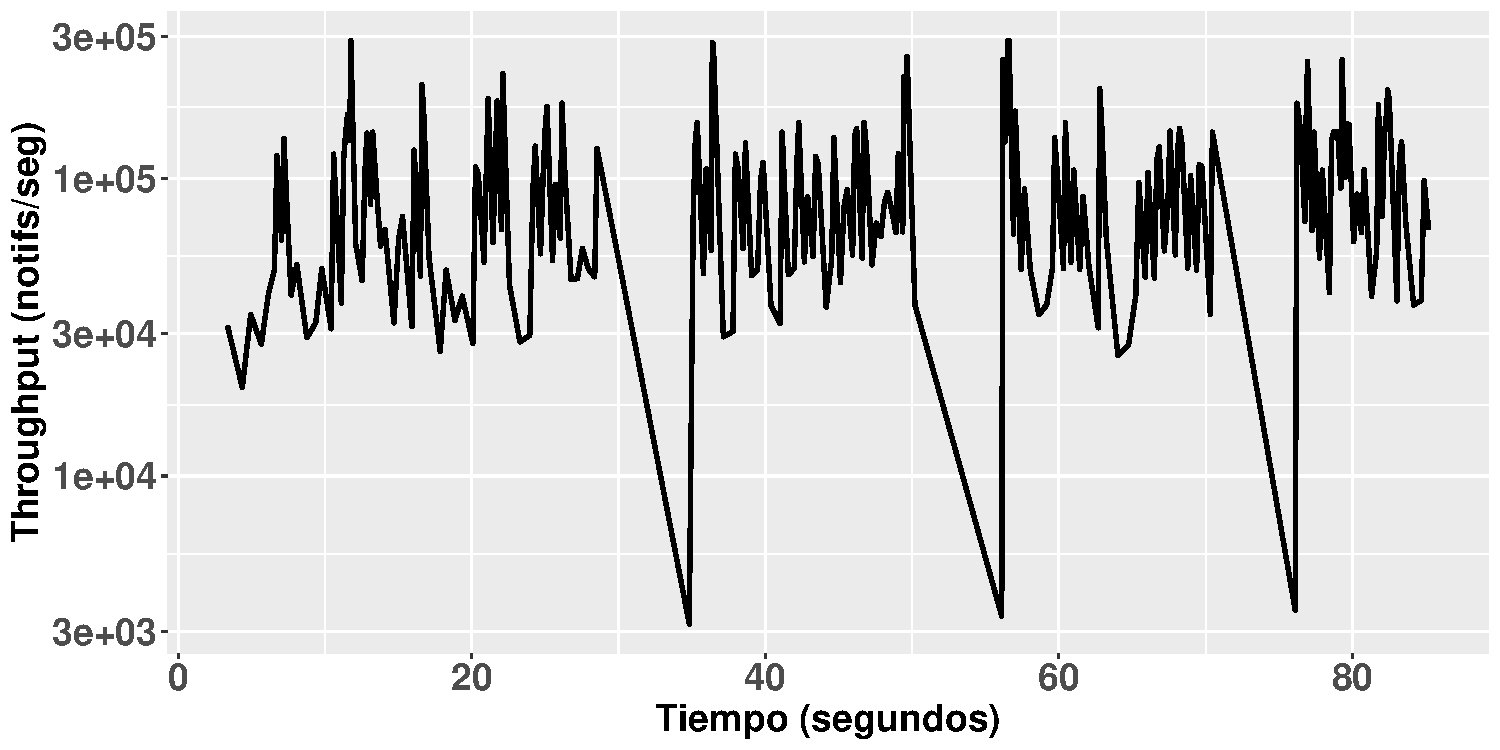
\includegraphics[width=\textwidth]{images/full-worklad-inc-msgrate/th_full-workload-inc-msgrate_1M.pdf}
    \caption{Throughput de prueba con carga completa e input rate de 1.000.000 mensajes/s.}
    \label{fig:fullworkload-inc-msgrate-th-1M}
\end{figure}

\begin{figure}[htpb]
    \centering
    \includegraphics[width=\textwidth]{images/full-worklad-inc-msgrate/rt_full-workload-inc-msgrate_1M.pdf}
    \caption{Tiempo de respuesta de prueba con carga completa e input rate de 1.000.000 mensajes/s.}
    \label{fig:fullworkload-inc-msgrate-rt-1M}
\end{figure}

%%%%%%%%%%%%%%%%%%%%%%%%%%%%%%%%%%%%%%%%%%%%%%%%%%%%%%%%%%%%%%%%%%%%%%%%%%%%%%%%

\subsubsection*{- 6.433.794 mensajes por segundo (máxima velocidad posible)}

Esta prueba presenta unos resultados similares a los resultados de las anteriores
pruebas (lo cual es esperable), con un throughput con caídas
(ver \autoref{fig:fullworkload-inc-msgrate-th-full}), que coinciden
con incrementos en el tiempo de respuesta (ver 
\autoref{fig:fullworkload-inc-msgrate-rt-full}), el cual presenta unos valores
en incremento, igual que en previas pruebas, llegando a los 85 segundos de tiempo
de respuesta.

Conclusiones de la prueba:
\begin{itemize}
    \item Viendo esta prueba y las anteriores, el throughput no supera los
    300.000, y en este caso, solo supera los 200.000 en ciertos picos, precedidos
    de valles (notificaciones encoladas que se procesan a gran velocidad).
    \item El tiempo de respuesta presenta unos valores en incremento, lo que concuerda
    con los valores del throughput, y con la propia saturación del sistema.
\end{itemize}

\begin{figure}[htpb]
    \centering
    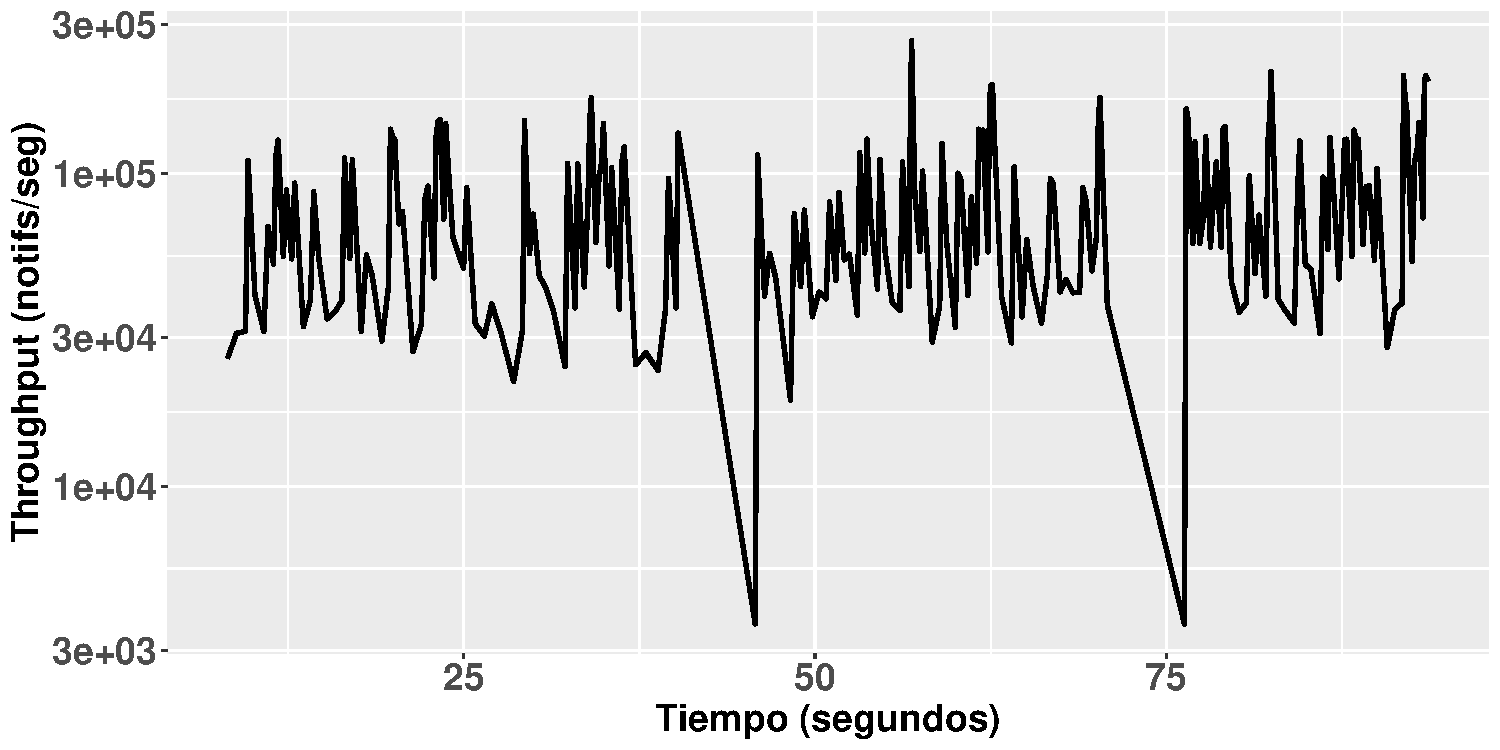
\includegraphics[width=\textwidth]{images/full-worklad-inc-msgrate/th_full-workload-inc-msgrate_full.pdf}
    \caption{Throughput de prueba con carga completa a máximo input rate.}
    \label{fig:fullworkload-inc-msgrate-th-full}
\end{figure}

\begin{figure}[htpb]
    \centering
    \includegraphics[width=\textwidth]{images/full-worklad-inc-msgrate/rt_full-workload-inc-msgrate_full.pdf}
    \caption{Tiempo de respuesta de prueba con carga completa a máximo input rate.}
    \label{fig:fullworkload-inc-msgrate-rt-full}
\end{figure}

%%%%%%%%%%%%%%%%%%%%%%%%%%%%%%%%%%%%%%%%%%%%%%%%%%%%%%%%%%%%%%%%%%%%%%%%%%%%%%%%

\subsection*{Secuencia logarítmica de subscripciones}

Como se puede observar en la \autoref{fig:throughput_logsubs}, el throughput 
del sistema decae de forma considerable pasadas las 20.000 subscripciones 
activas, ya que el tiempo invertido en comprobar todas las subscripciones 
incrementa y provoca un aumento en el tiempo de procesado de cada publicación,
en concreto, en la confección de la lista de subscripciones interesadas en
dicha publicación.

Esto indica que con la configuración actual (1-1-1), el sistema está saturando
cuando tiene que comprobar, al menos, 20.000 subscripciones. En este punto, si
estuviese activada la escalabilidad, el sistema debería de haber escalado para
no llegar a saturar.

\begin{figure}[htpb]
    \centering
    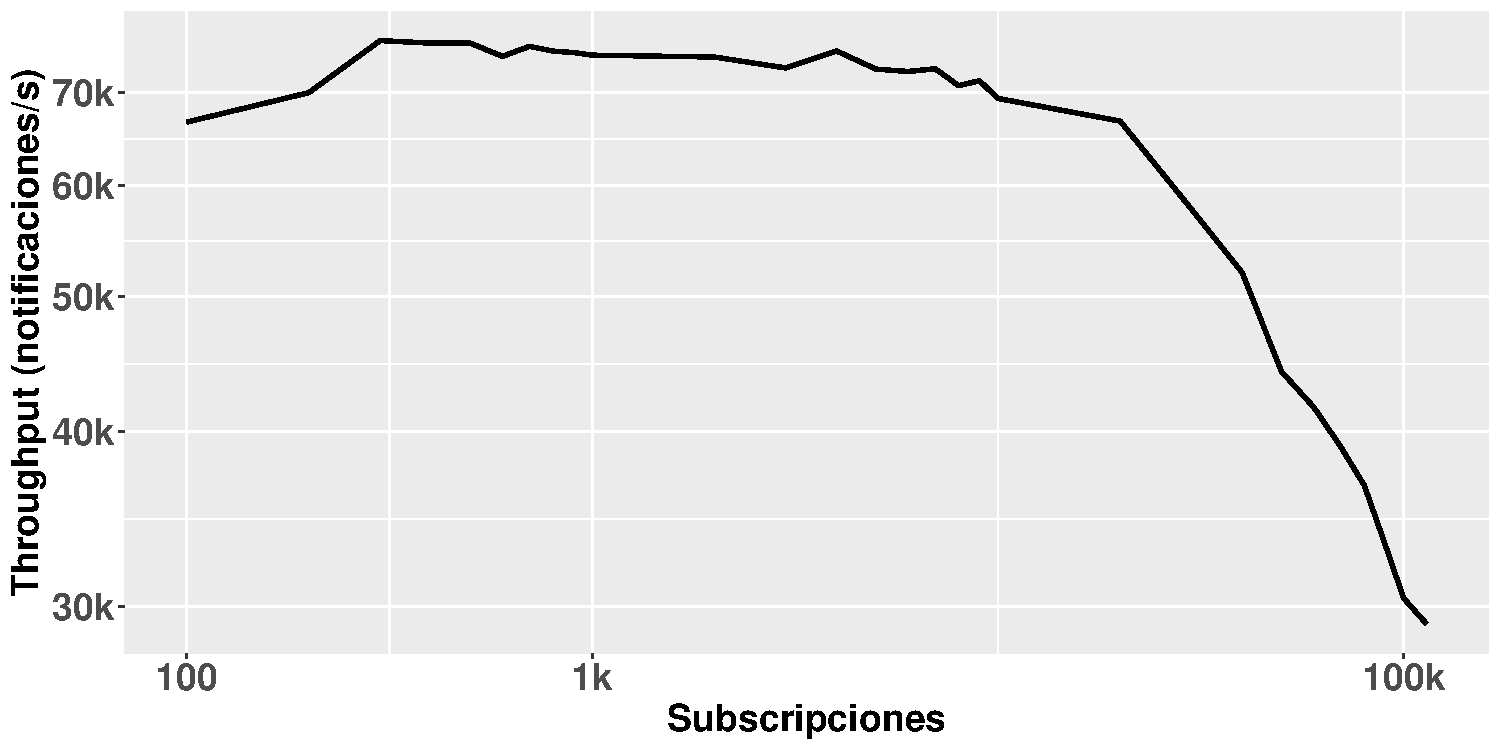
\includegraphics[width=\textwidth]{images/log-subs/throughput_logsubs_IR-100k.pdf}
    \caption{Throughput en base a la subscripciones activas con un input rate de 100.000 mensajes por segundo en ejes logarítmicos.}
    \label{fig:throughput_logsubs}
\end{figure}

Conociendo este punto de saturación, lo siguiente es probar el sistema con esa
carga de subscripciones, de forma que se vea con mayor precisión cómo actúa el
sistema con un número de subscripciones cercano al del punto de saturación.

%%%%%%%%%%%%%%%%%%%%%%%%%%%%%%%%%%%%%%%%%%%%%%%%%%%%%%%%%%%%%%%%%%%%%%%%%%%%%%%%

\subsection*{Carga de subscripciones creciente}

Como se puede observar en la \autoref{fig:throughput_incsubsload-fullpubs}, el
throughput del sistema cae en gran medida, con una media de 18.000 mensajes 
por segundo, con picos cercanos a los 30.000.

Este primer pico se debe al aumento de subscripciones, que provocan que las 
publicaciones enviadas de forma paralela generen un mayor número de notificaciones,
lo cual aumenta el número de notificaciones generadas por segundo.

De igual forma, estos picos pueden estar causados por la naturaleza de la
distribución de subscripciones y publicaciones, ya que ciertas secciones de la 
carga de publicaciones pueden generar mayor número de notificaciones, al
machear con más subscripciones activas.

A causa de esto, se requiere de realizar nuevas pruebas con otro tipo de
carga de trabajo, que pruebe la saturación del sistema con incrementos puntuales,
como se puede esperar en un contexto real.

\begin{figure}[htpb]
    \centering
    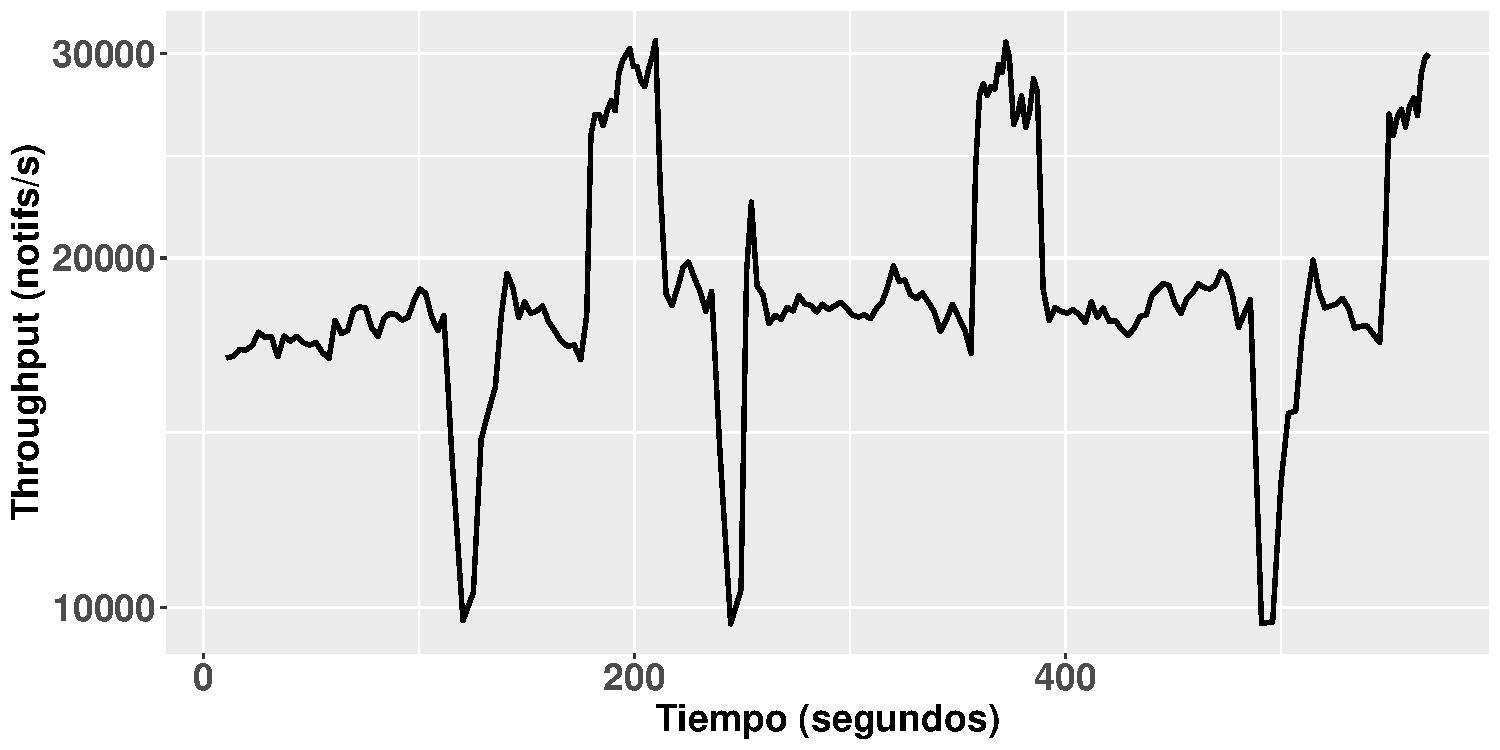
\includegraphics[width=\textwidth]{images/throughput_inc-subs-load-full.pdf}
    \caption{Throughput del sistema con la carga de subscripciones y todas las publicaciones}
    \label{fig:throughput_incsubsload-fullpubs}
\end{figure}


%%%%%%%%%%%%%%%%%%%%%%%%%%%%%%%%%%%%%%%%%%%%%%%%%%%%%%%%%%%%%%%%%%%%%%%%%%%%%%%%

\subsection*{Carga de subscripciones estática}

\subsubsection*{- 50.000 subscripciones}

En la \autoref{fig:subsworkload_50k-200k} se puede observar la caída de rendimiento
del sistema, pues ha llegado al punto de saturación parcial al caer este muy por debajo
del throughput esperado de 200.000 mensajes por segundo. Las fluctuaciones 
indican que el sistema, en ciertos momentos, encola gran cantidad de eventos, al
no poder procesarlos a tiempo, pero recupera ese tiempo perdido en los siguientes
segundos. A pesar de esto, el sistema no llega a saturar de la forma esperada, es decir,
se recupera más rápido de lo esperado, lo cual es bueno para el sistema, pero no nos 
proporciona la información buscada.

\begin{figure}[htpb]
    \centering
    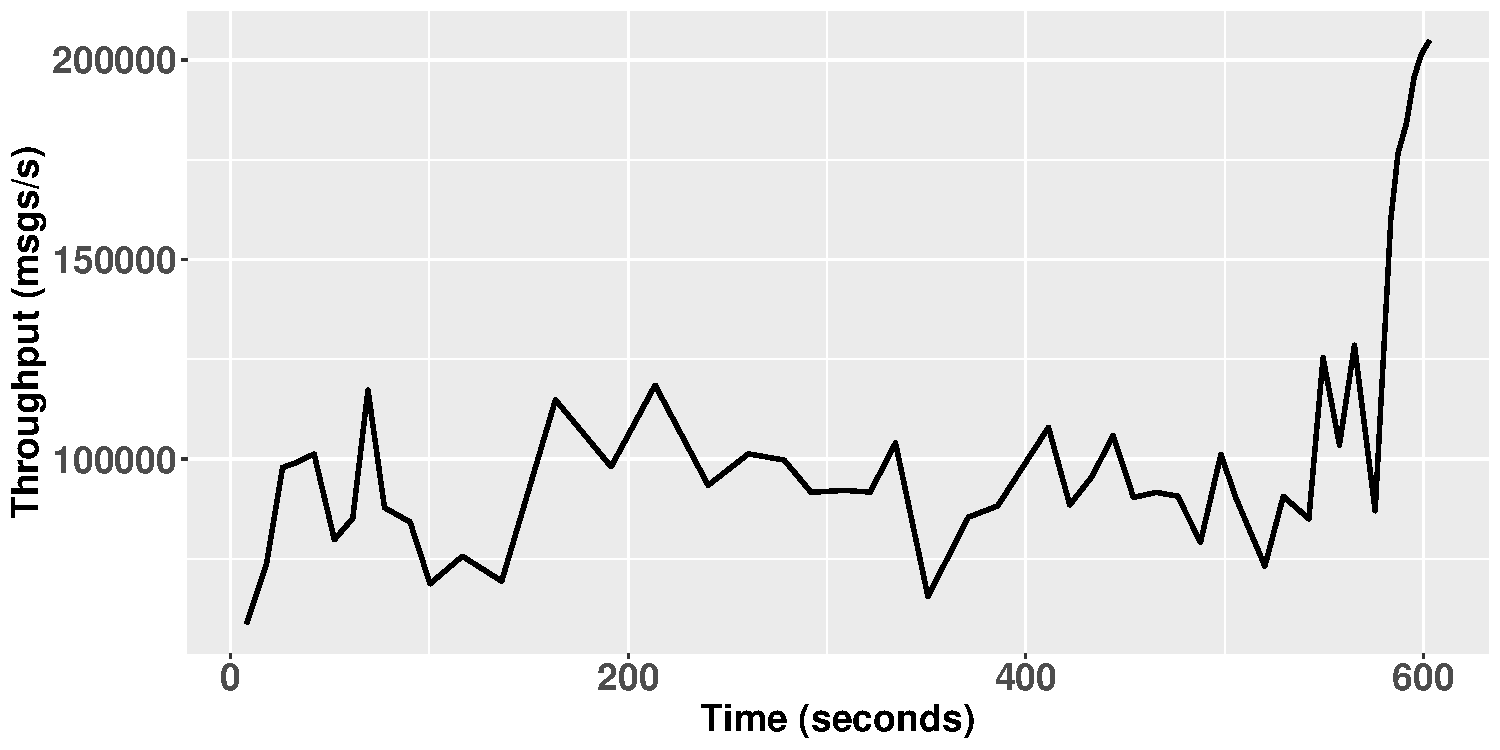
\includegraphics[width=\textwidth]{images/th_subs_workload-50k-200k.pdf}
    \caption{Throughput resultante de una prueba con 50.000 subscripciones y un input rate de 200.000 publicaciones por segundo.}
    \label{fig:subsworkload_50k-200k}
\end{figure}

\subsubsection*{- 100.000 subscripciones}

Si se lleva esta prueba al límite, es decir, el caso máximo en el cual dicha prueba puede
acabar sin quedarse el ordenador sin memoria para llevarla a cabo, se puede observar
la inestabilidad del rendimiento del sistema, al haber este saturado de forma parcial.
Esto se puede observar en la \autoref{fig:subsworkload_100k-200k}.

\begin{figure}[htpb]
    \centering
    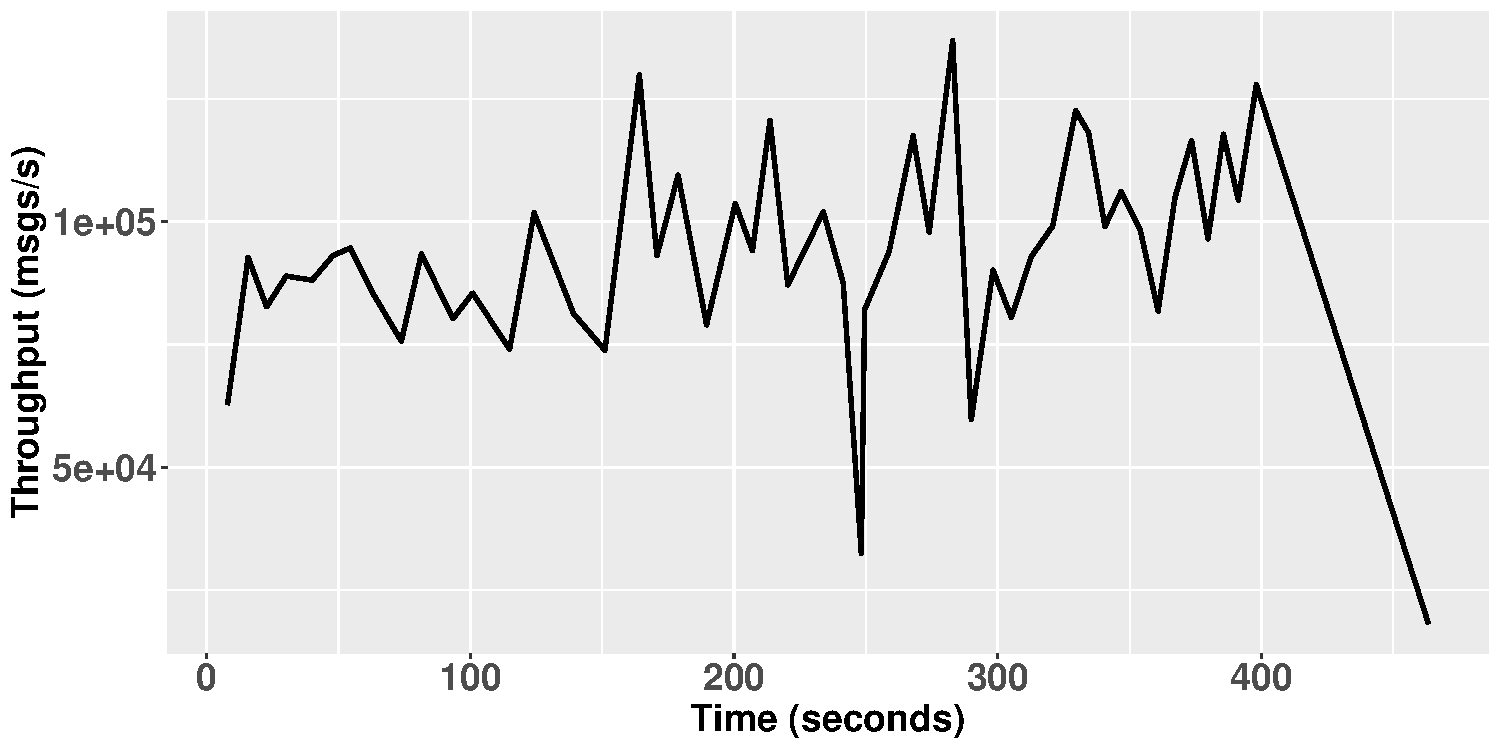
\includegraphics[width=\textwidth]{images/th_subs_workload-100k-200k.pdf}
    \caption{Throughput resultante de una prueba con 100000 subscripciones y un input rate de 200.000 publicaciones por segundo.}
    \label{fig:subsworkload_100k-200k}
\end{figure}

Los resultados obtenidos mediante estas pruebas nos muestran que el sistema satura
parcialmente de forma efectiva con una carga de 100.000 subscripciones y un input rate
mayor o igual a 150.000 mensajes por segundo. Esta respuesta nos ayuda a encontrar, con
mayor precisión, pero para ello se han de poner en práctica más pruebas con diferentes
cargas.

\subsection*{Carga de subscripciones con crecimiento puntual}

\subsubsection*{Crecimiento de 20.000 a 100.000 subscripciones}

Siguiendo el modelo de pruebas previamente empleado, mediante aplicar carga 
representada por la \autoref{fig:subsworkload_20k-100k}, y especificando un 
input rate fijo de 125.000 mensajes por segundo, se ha obtenido el throughput
que se muestra en la \autoref{fig:subsworkload_spike_20k-100k-125k}.

\begin{figure}[htpb]
    \centering
    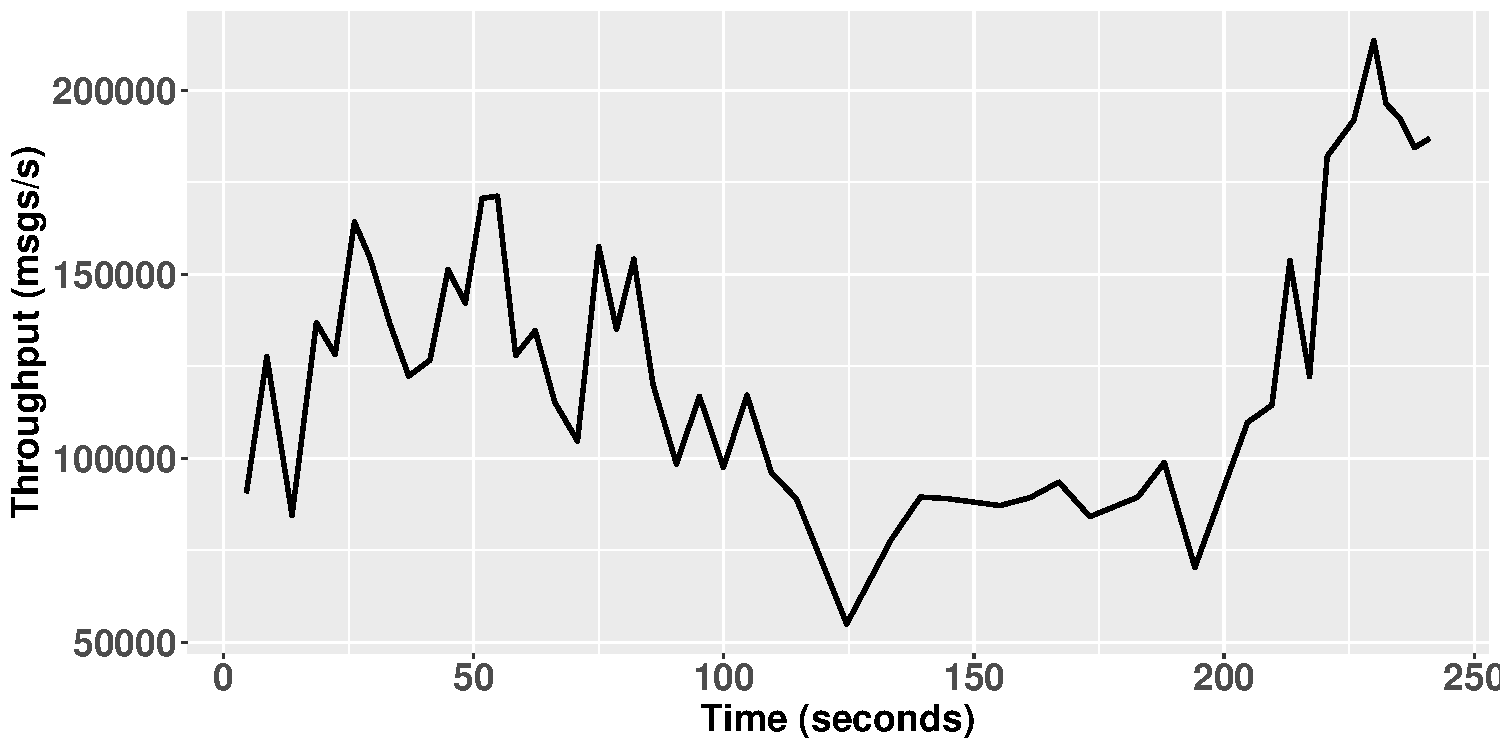
\includegraphics[width=\textwidth]{images/throguhput_spike_20k-100k-125k.pdf}
    \caption{Throughput resultante de la carga de la \autoref{fig:subsworkload_20k-100k} e input rate de 125.000 publicaciones por segundo.}
    \label{fig:subsworkload_spike_20k-100k-125k}
\end{figure}

El throughput de la \autoref{fig:subsworkload_spike_20k-100k-125k} demuestra que
el sistema ha saturado parcialmente, y ha llegado a recuperarse en la segunda mitad
de la prueba, llegando a un throughput de 125.000, al haber encolado gran cantidad de
mensajes. Junto con esto, se aprecia un throughput muy inestable, con muchos picos
bajos y altos. Los valores proporcionados para esta prueba son los más altos posibles,
sin que la ordenador se quede sin memoria para poder llevar a cabo esta, por lo que
sabemos que el sistema satura de forma efectiva a partir de estos valores.

\subsubsection*{Crecimiento de 25.000 a 100.000 subscripciones}

A raíz de estos resultados, se ha desarrollado la carga representada por la 
\autoref{fig:subsworkload_25k-113k} que resulta en el throughput representado por 
la \autoref{fig:subsworkload_spike_25k-113k-125k}.

\begin{figure}[htpb]
    \centering
    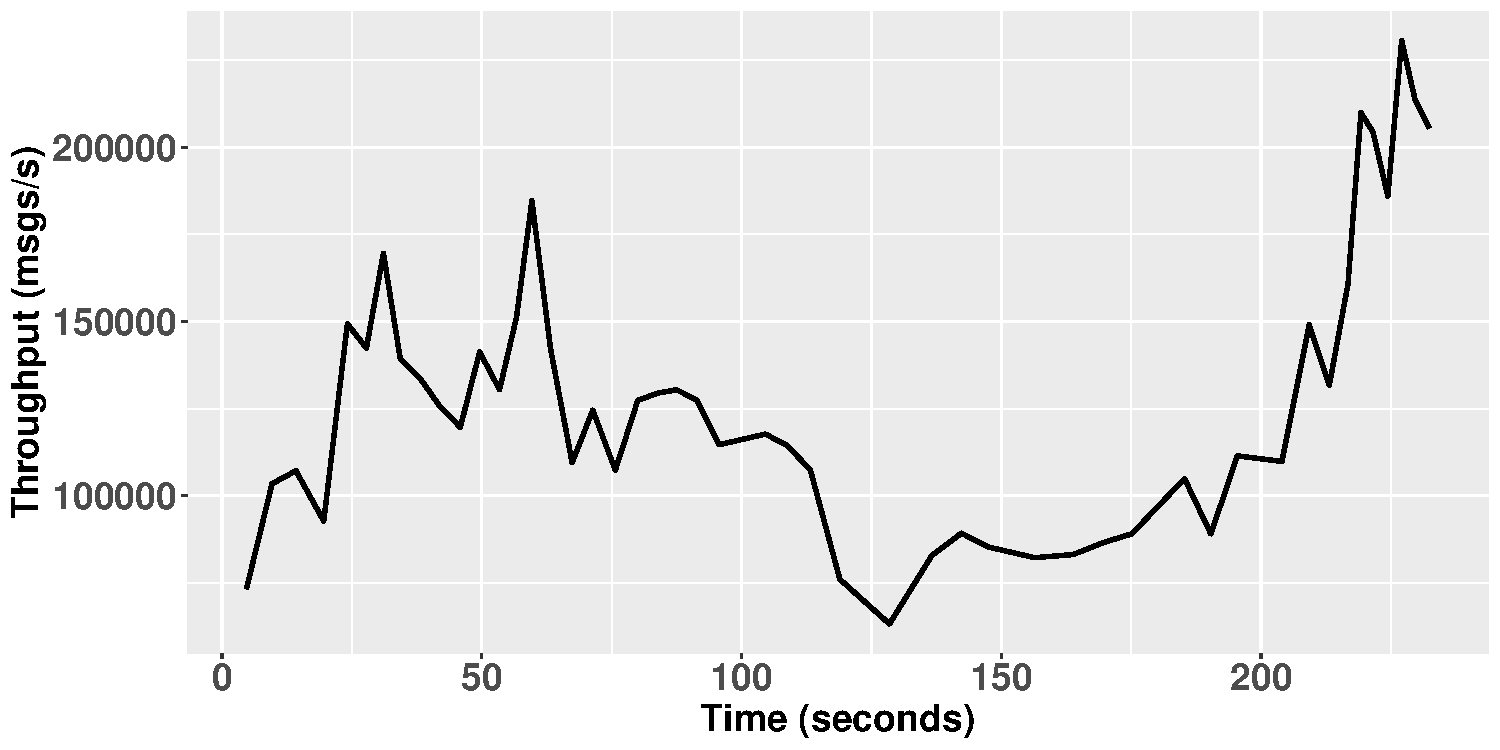
\includegraphics[width=\textwidth]{images/throguhput_spike_20k-113k-125k.pdf}
    \caption{Throughput resultante de la carga de la \autoref{fig:subsworkload_25k-113k} e input rate de 125.000 publicaciones por segundo.}
    \label{fig:subsworkload_spike_25k-113k-125k}
\end{figure}

Dados estos resultados, el comportamiento del sistema con estas pruebas no es el óptimo
para aplicar estos valores a los modelos predictivos. A causa de esto, se ha desarrollado
una prueba adicional, similar a las anteriores, pero que implementa un incremento más
repentino (llegar al máximo en 2-3 segundos) con un menor input ratio, de forma que el
sistema sature parcialmente en el punto del incremento, pero sea capaz de recuperarse
a tiempo.

\subsubsection*{Crecimiento rápido de 25.000 a 113.904 subscripciones}

Los resultados de esta prueba, que sigue los mismos parámetros que la anterior pero con un
input ratio de 100.000 mensajes por segundo, se pueden observar en la
\autoref{fig:subsworkload_th_fast_spike_25k-113k-100k}, que muestra una saturación muy leve del
sistema cuando se alcanza el incremento de la carga, pero en sistema se recupera en muy poco tiempo.

Este resultado, a pesar de haber saturado de forma mínima el sistema, es el buscado, pues el
throughput del sistema es estable y el sistema satura de la forma esperada, a pesar de haberse
recuperado rápidamente.

\begin{figure}[htpb]
    \centering
    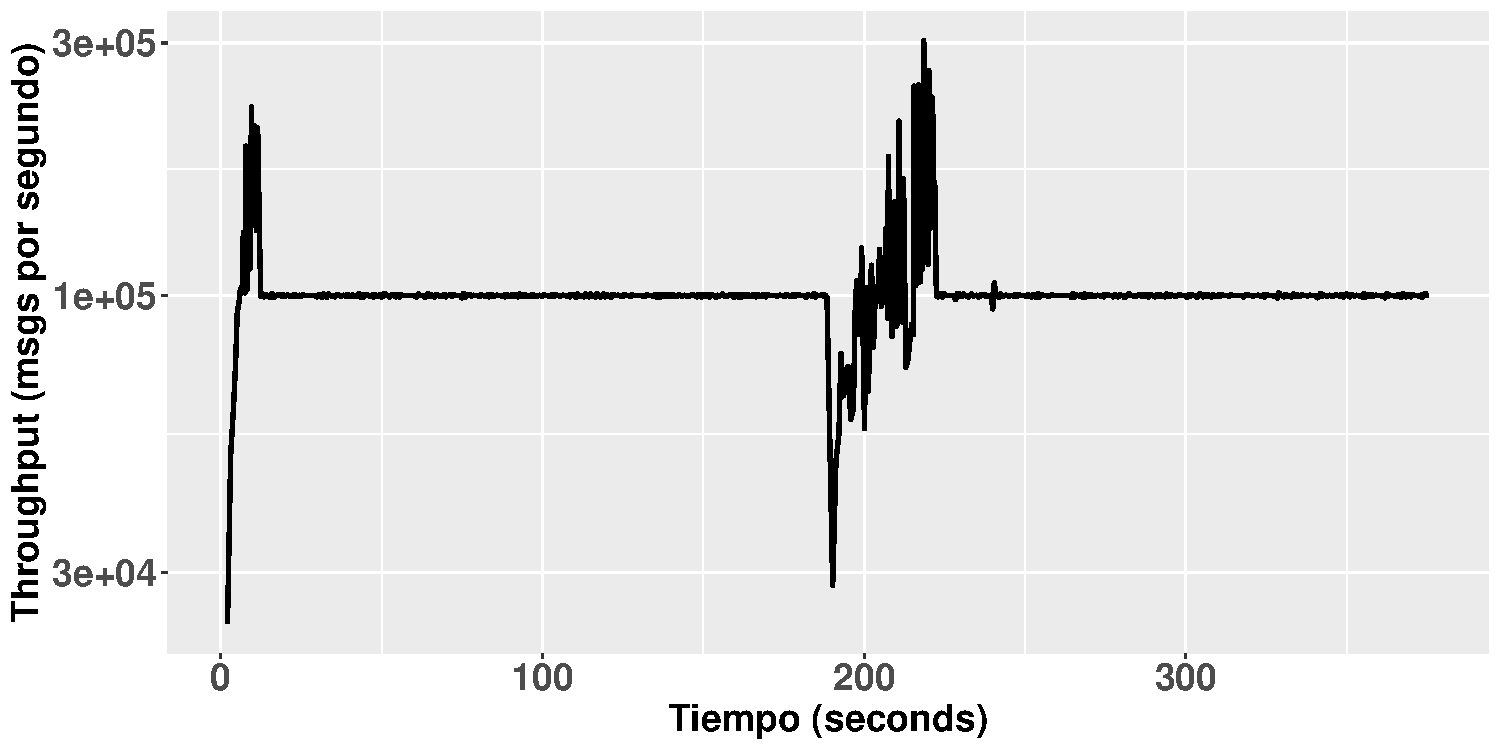
\includegraphics[width=\textwidth]{images/th_test_spike_25k-113k_100000.pdf}
    \caption{Throughput resultante de la carga de la \autoref{fig:subsworkload_fast_spike_25k-113k-100k} e input rate de 100.000 publicaciones por segundo.}
    \label{fig:subsworkload_th_fast_spike_25k-113k-100k}
\end{figure}

Habiendo obtenido estos resultados, que simulan diferentes situaciones
reales, podemos usar estos para aplicar los modelos predictivos, una vez
desarrollados e implementados estos. Los modelos predictivos usarán estos 
resultados para llevar a cabo dichas predicciones, para que el sistema pueda
anticiparse a cualquier situación que sea posible predecir.